% Template for PLoS
% Version 3.5 March 2018
%
% % % % % % % % % % % % % % % % % % % % % %
%
% -- IMPORTANT NOTE
%
% This template contains comments intended 
% to minimize problems and delays during our production 
% process. Please follow the template instructions
% whenever possible.
%
% % % % % % % % % % % % % % % % % % % % % % % 
%
% Once your paper is accepted for publication, 
% PLEASE REMOVE ALL TRACKED CHANGES in this file 
% and leave only the final text of your manuscript. 
% PLOS recommends the use of latexdiff to track changes during review, as this will help to maintain a clean tex file.
% Visit https://www.ctan.org/pkg/latexdiff?lang=en for info or contact us at latex@plos.org.
%
%
% There are no restrictions on package use within the LaTeX files except that 
% no packages listed in the template may be deleted.
%
% Please do not include colors or graphics in the text.
%
% The manuscript LaTeX source should be contained within a single file (do not use \input, \externaldocument, or similar commands).
%
% % % % % % % % % % % % % % % % % % % % % % %
%
% -- FIGURES AND TABLES
%
% Please include tables/figure captions directly after the paragraph where they are first cited in the text.
%
% DO NOT INCLUDE GRAPHICS IN YOUR MANUSCRIPT
% - Figures should be up\textit{loaded} separately from your manuscript file. 
% - Figures generated using LaTeX should be extracted and removed from the PDF before submission. 
% - Figures containing multiple panels/subfigures must be combined into one image file before submission.
% For figure citations, please use "Fig" instead of "Figure".
% See http://journals.plos.org/plosone/s/figures for PLOS figure guidelines.
%
% Tables should be cell-based and may not contain:
% - spacing/line breaks within cells to alter layout or alignment
% - do not nest tabular environments (no tabular environments within tabular environments)
% - no graphics or colored text (cell background color/shading OK)
% See http://journals.plos.org/plosone/s/tables for table guidelines.
%
% For tables that exceed the width of the text column, use the adjustwidth environment as illustrated in the example table in text below.
%
% % % % % % % % % % % % % % % % % % % % % % % %
%
% -- EQUATIONS, MATH SYMBOLS, SUBSCRIPTS, AND SUPERSCRIPTS
%
% IMPORTANT
% Below are a few tips to help format your equations and other special characters according to our specifications. For more tips to help reduce the possibility of formatting errors during conversion, please see our LaTeX guidelines at http://journals.plos.org/plosone/s/latex
%
% For inline equations, please be sure to include all portions of an equation in the math environment.  For example, x$^2$ is incorrect; this should be formatted as $x^2$ (or $\mathrm{x}^2$ if the romanized font is desired).
%
% Do not include text that is not math in the math environment. For example, CO2 should be written as CO\textsubscript{2} instead of CO$_2$.
%
% Please add line breaks to long display equations when possible in order to fit size of the column. 
%
% For inline equations, please do not include punctuation (commas, etc) within the math environment unless this is part of the equation.
%
% When adding superscript or subscripts outside of brackets/braces, please group using {}.  For example, change "[U(D,E,\gamma)]^2" to "{[U(D,E,\gamma)]}^2". 
%
% Do not use \cal for caligraphic font.  Instead, use \mathcal{}
%
% % % % % % % % % % % % % % % % % % % % % % % % 
%
% Please contact latex@plos.org with any questions.
%
% % % % % % % % % % % % % % % % % % % % % % % %

\documentclass[10pt,letterpaper]{article}
\usepackage[top=0.85in,left=2.75in,footskip=0.75in]{geometry}

% customized packages
\usepackage{fixltx2e}
\usepackage{stfloats}
\usepackage{subfloat}
\usepackage[caption=false,font=footnotesize]{subfig}

% amsmath and amssymb packages, useful for mathematical formulas and symbols
\usepackage{amsmath,amssymb}
% algorithm,algorithmicx,algpseudocode are used for writing pseudo code and algorithms
\usepackage{algorithm,algorithmicx,algpseudocode}
% multirow is used for adjusting the table
\usepackage{multirow}
% Use adjustwidth environment to exceed column width (see example table in text)
\usepackage{changepage}

% Use Unicode characters when possible
\usepackage[utf8x]{inputenc}

% textcomp package and marvosym package for additional characters
\usepackage{textcomp,marvosym}

% cite package, to clean up citations in the main text. Do not remove.
\usepackage{cite}

% Use nameref to cite supporting information files (see Supporting Information section for more info)
\usepackage{nameref,hyperref}

% line numbers
\usepackage[right]{lineno}

% ligatures disabled
\usepackage{microtype}
\DisableLigatures[f]{encoding = *, family = * }

% color can be used to apply background shading to table cells only
\usepackage[table]{xcolor}
\usepackage{booktabs}
% stop disconnecting vertical lines:
\setlength{\aboverulesep}{0ex}
\setlength{\belowrulesep}{0ex}
% array package and thick rules for tables
\usepackage{array}

% create "+" rule type for thick vertical lines
\newcolumntype{+}{!{\vrule width 2pt}}

% create \thickcline for thick horizontal lines of variable length
\newlength\savedwidth
\newcommand\thickcline[1]{%
	\noalign{\global\savedwidth\arrayrulewidth\global\arrayrulewidth 2pt}%
	\cline{#1}%
	\noalign{\vskip\arrayrulewidth}%
	\noalign{\global\arrayrulewidth\savedwidth}%
}

% \thickhline command for thick horizontal lines that span the table
\newcommand\thickhline{\noalign{\global\savedwidth\arrayrulewidth\global\arrayrulewidth 2pt}%
	\hline
	\noalign{\global\arrayrulewidth\savedwidth}}


% Remove comment for double spacing
%\usepackage{setspace} 
%\doublespacing

% Text layout
\raggedright
\setlength{\parindent}{0.5cm}
\textwidth 5.25in 
\textheight 8.75in

% Bold the 'Figure #' in the caption and separate it from the title/caption with a period
% Captions will be left justified
\usepackage[aboveskip=1pt,labelfont=bf,labelsep=period,justification=raggedright,singlelinecheck=off]{caption}
\renewcommand{\figurename}{Fig}

% Use the PLoS provided BiBTeX style
\bibliographystyle{plos2015}

% Remove brackets from numbering in List of References
\makeatletter
\renewcommand{\@biblabel}[1]{\quad#1.}
\makeatother



% Header and Footer with logo
\usepackage{lastpage,fancyhdr,graphicx}
\usepackage{epstopdf}
\graphicspath{{../../Figures/}}
\renewcommand{\thefigure}{C\arabic{figure}}
%\pagestyle{myheadings}
\pagestyle{fancy}
\fancyhf{}
%\setlength{\headheight}{27.023pt}
%\lhead{\includegraphics[width=2.0in]{PLOS-submission.eps}}
\rfoot{\thepage/\pageref{LastPage}}
\renewcommand{\headrulewidth}{0pt}
\renewcommand{\footrule}{\hrule height 2pt \vspace{2mm}}
\fancyheadoffset[L]{2.25in}
\fancyfootoffset[L]{2.25in}
\lfoot{\today}

%% Include all macros below

\newcommand{\lorem}{{\bf LOREM}}
\newcommand{\ipsum}{{\bf IPSUM}}

%% END MACROS SECTION


\begin{document}
\vspace*{0.2in}
	
{\Large\textbf\newline{{Supporting Document for Studied Specific Cases}} % Please use "sentence case" for title and headings (capitalize only the first word in a title (or heading), the first word in a subtitle (or subheading), and any proper nouns).
}
\\
\vspace{5 mm}
We conducted four different case studies to get more insight into the performance of assistive devices that include studying both assistive devices in a particular load condition or an assistive device in two different load conditions with the same effect on the metabolic power expenditure or the same power consumption of assistive actuators. Investigating these specific configurations of the optimal devices helped us to understand how the profiles of devices with the same performances change in a load condition more systematically. These cases can also help us to gain insight into the effect of load condition on an assistive device profiles, and clarify how a particular device can be affected by loading assisted subjects with a heavy load.
\begin{figure*}[!ht]   
	\centering
	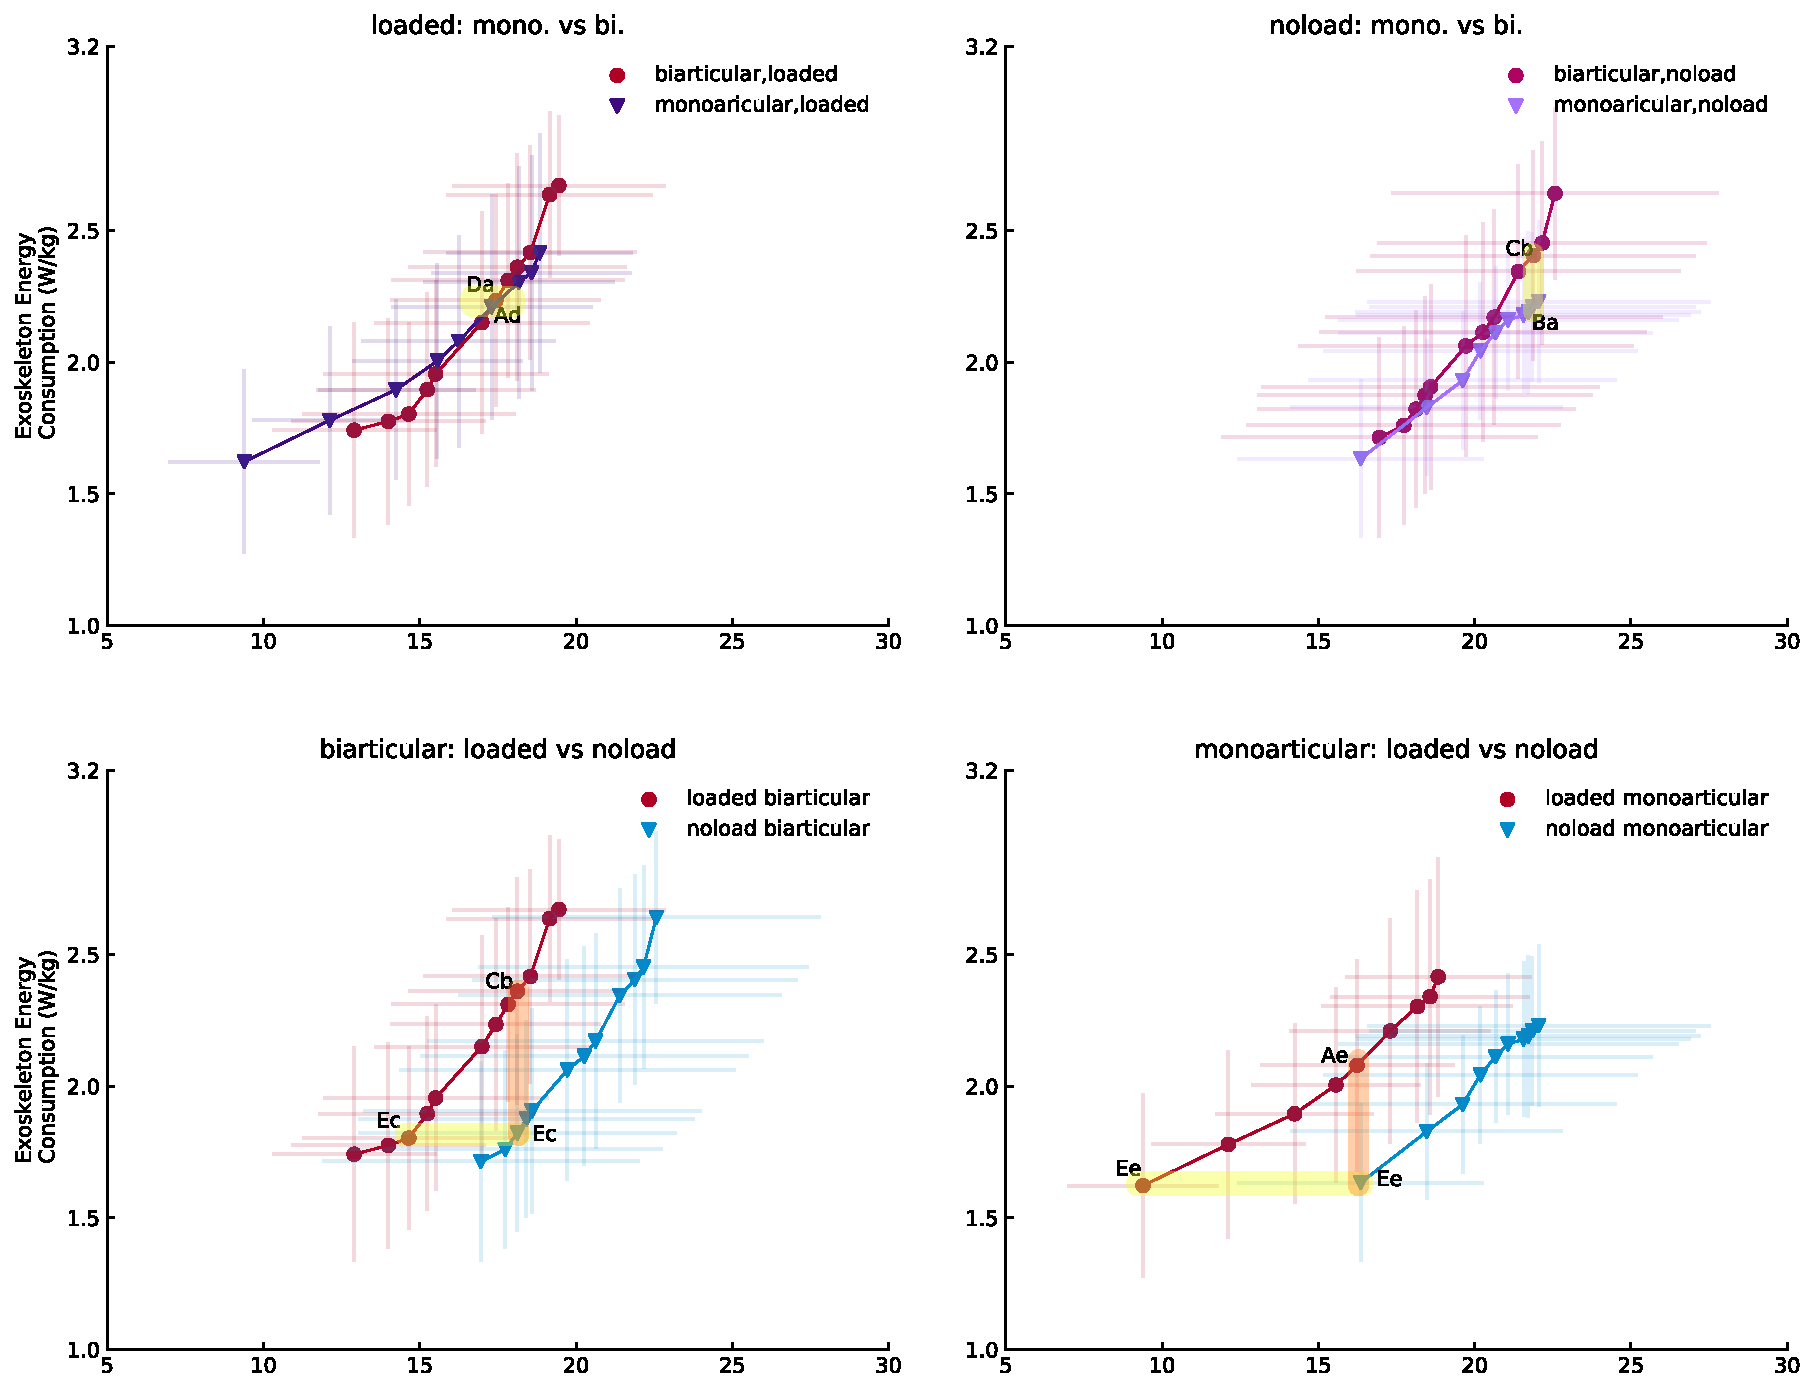
\includegraphics[width=\linewidth]{Case_Studies/PaperFigure_Selected_Configurations.pdf}
	\vspace{1mm}
	\caption{{\small\textbf{Studied cases chosen from the Pareto front curves.} The chosen optimal solutions of each configuration in each of both load conditions used to be studied. The selected solutions on Pareto front curves are resulted from averaging over 7 subjects and 3 trials.}}
	\label{Fig_Selected_OptimalDevices_On_Pareto}
\end{figure*}
%%%%%%%%%%%%%%%%%%%%%%%%%%%%%%%%%%%%%%%%%%%%%%%%%%%%%%%%%%%%%%%%%%%%%%%%%%%%%%%%%%%%%%%%%%%%%%%%%%%%%%%%%%%%%%%%%%%%
\section*{Case 1: Devices Performance in \textit{loaded} Condition}
It was shown that the optimal trade-offs of both exoskeletons are practically the same in the {\it loaded} condition. To study the performance of each actuator of the devices, and their effect on the muscle activity of assisted subjects, we selected two devices on Pareto front that had nearly the same performance in both metabolic cost reduction and power consumption. The chosen device for monoarticular has 70 N.m hip peak torque and 40 N.m knee peak torque, which is represented by "Ad" on Pareto front ( Figure \ref{Fig_Selected_OptimalDevices_On_Pareto}), and the peak torques of the biarticular device are 40, and 70 N.m on hip and knee, respectively, represented with "Da " on the Pareto front. As can be inferred from the configurations of devices, although these two chosen devices have the same performance on defined objectives, they have a completely different arrangement on hip and knee actuators.
\begin{figure*}[ht]   
	\centering
	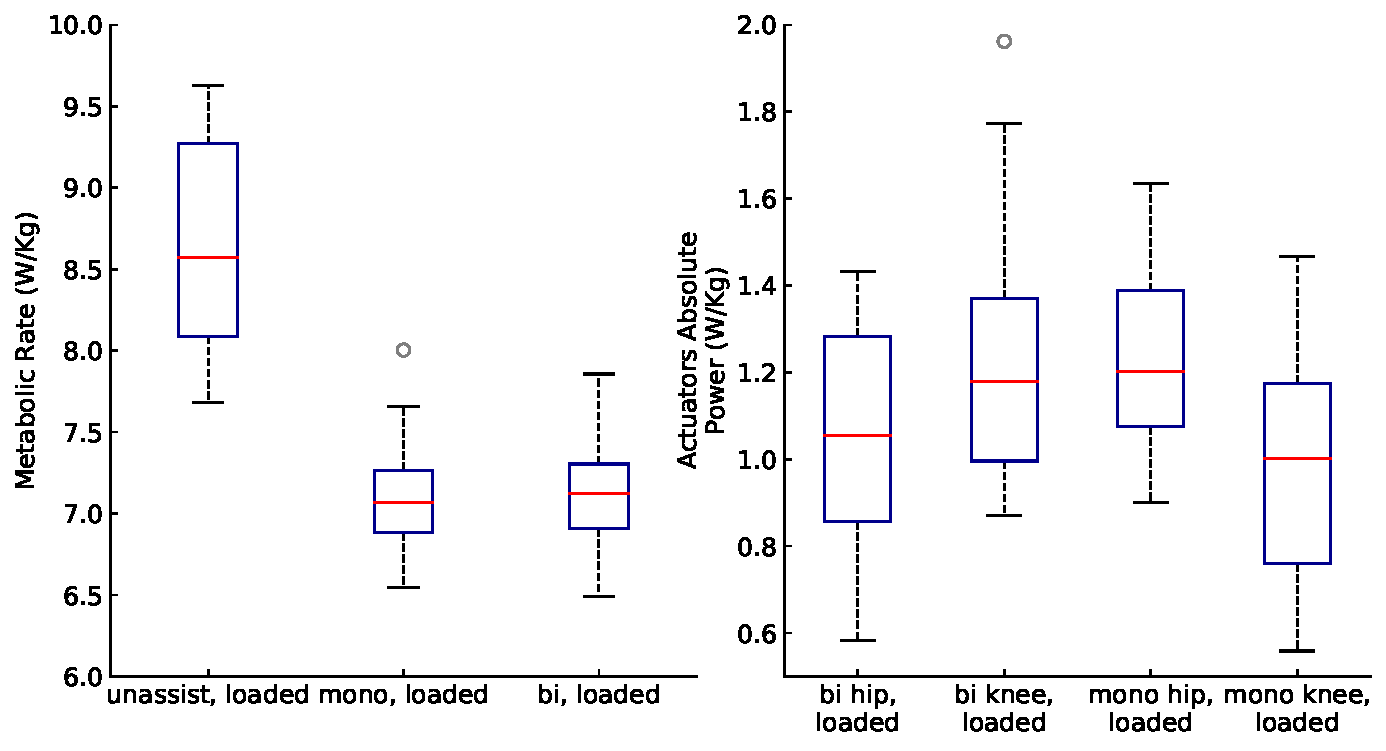
\includegraphics[width=\linewidth]{Case_Studies/LoadedMono04_LoadedBi16/PaperFigure_BoxPlot.pdf}
	\vspace{1mm}
	\caption{\small{\textbf{Assistive devices power consumption and their effect on the metabolic rate.} The power consumptions of assistive devices and their effect on whole-body metabolic rate of the subjects walking at self-selected speed while carrying a heavy load. Asterisks indicate statistically significant differences ( 7 subjects, 3 trails, Tukey Post-hoc, $P < 0.05$).}}
	\label{Fig_Case01_Energy_Plot}
\end{figure*}
The metabolic rate of assisted subjects with biarticular and monoarticular devices shows no significant difference between the amount of assistance delivered by these devices, which was expected from the Pareto front. While the total power consumptions of these two devices were practically identical on the Pareto front, the power consumption of the hip and knee actuators between the biarticular and monoarticular devices were statistically significantly different, as represented in Figure \ref{Fig_Case01_Energy_Plot}. This difference indicates that while the devices deliver the same assistance to the subjects carrying a heavy load, their assistance strategies are different, and this claim can be more illuminated by analyzing the profiles of actuators.\\
Although the selected monoarticular and biarticular exoskeletons have the same effect on the metabolic rate of {\it loaded} subjects, it was shown that their assistive actuator configurations were different, resulted in significantly different power consumption of actuators. This difference in the configuration of their actuators affects their mechanical design, especially their required gear train and reflected inertia. We employed the developed modified augmentation factor to assess the performance of the biarticular and monoarticular exoskeletons under the effect of device inertial properties. The computed modified augmentation factors for the monoarticular and biarticular devices were 0.66 $\pm$ 1.00 and  1.98 $\pm$ 0.71 W/kg, respectively, which indicates that both exoskeletons would be able to deliver assistance to the subjects even under inertial properties of devices, causing more metabolic burden on the subject. Additionally, the MAF values show that the biarticular device had superior performance to the monoarticular exoskeleton and the reason for this issue rooted in the mass distribution and gear train of the monoarticular device. The inertia calculations show the monoarticular device had practically three times more inertia on the thigh than the biarticular device, and according to the inertia location factor of the thigh, the effect of inertia on the thigh is expensive in terms of the metabolic rate increase which results in a lower MA factor for the monoarticular exoskeleton.\\
\begin{figure*}[ht]   
	\centering
	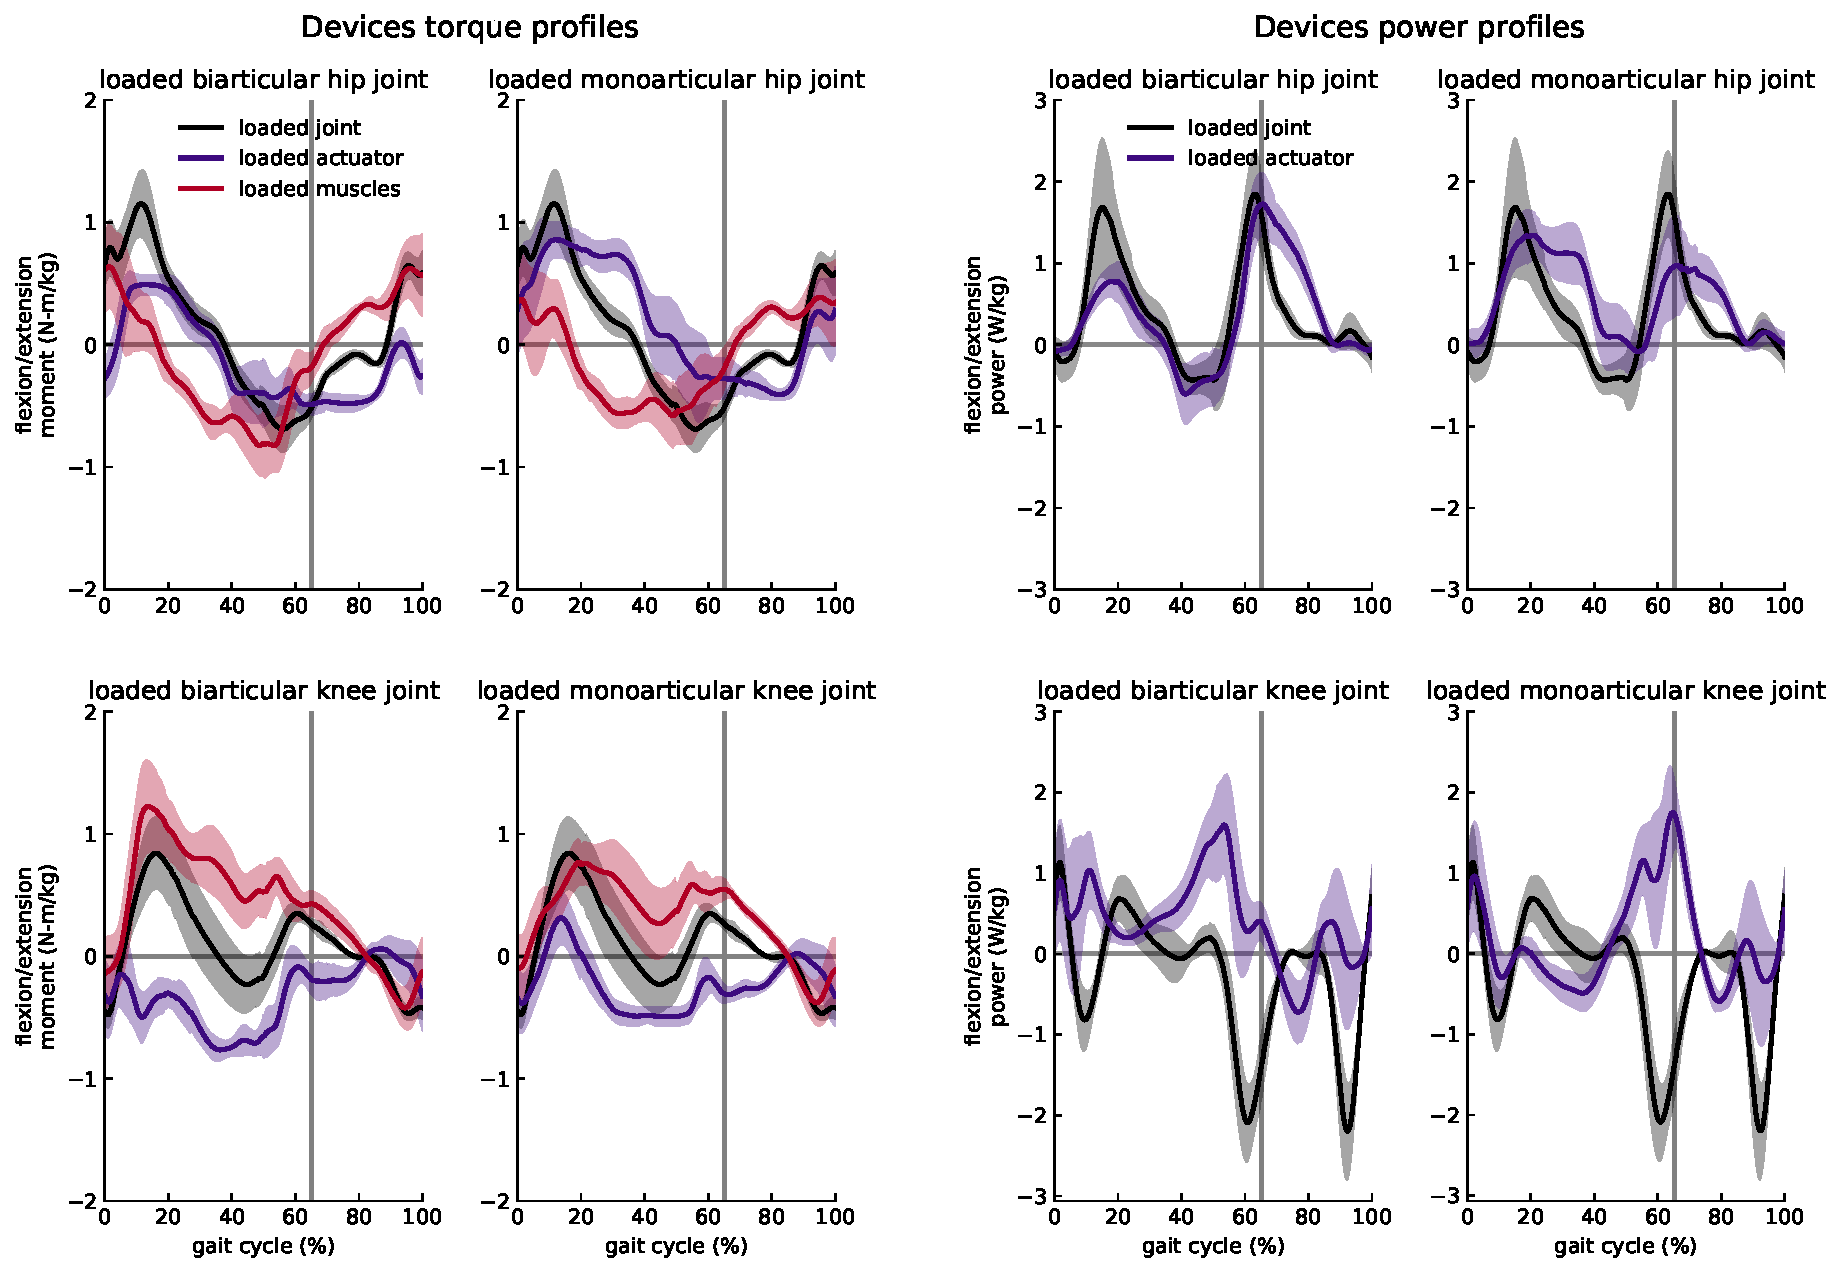
\includegraphics[width=\linewidth]{Case_Studies/LoadedMono04_LoadedBi16/PaperFigure_Profiles.pdf}
	\vspace{1mm}
	\caption{{\small\textbf{Assistive devices torque and power profiles.} The actuator torque and power for subjects carrying heavy load (dark purple) , and net joint power and torque profile for \textit{loaded} (black) condition are shown for each actuator of the devices. The torque profile of moment generated by muscles (dark red) is shown for each joint for both devices. The curves are averaged over 7 subjects with 3 trials and normalized by subject mass; shaded regions around the mean profile indicate standard deviation of the profile.}}
	\label{Fig_Case01_Torque_Power_Profiles}
\end{figure*}
\begin{figure*}[ht]   
	\centering
	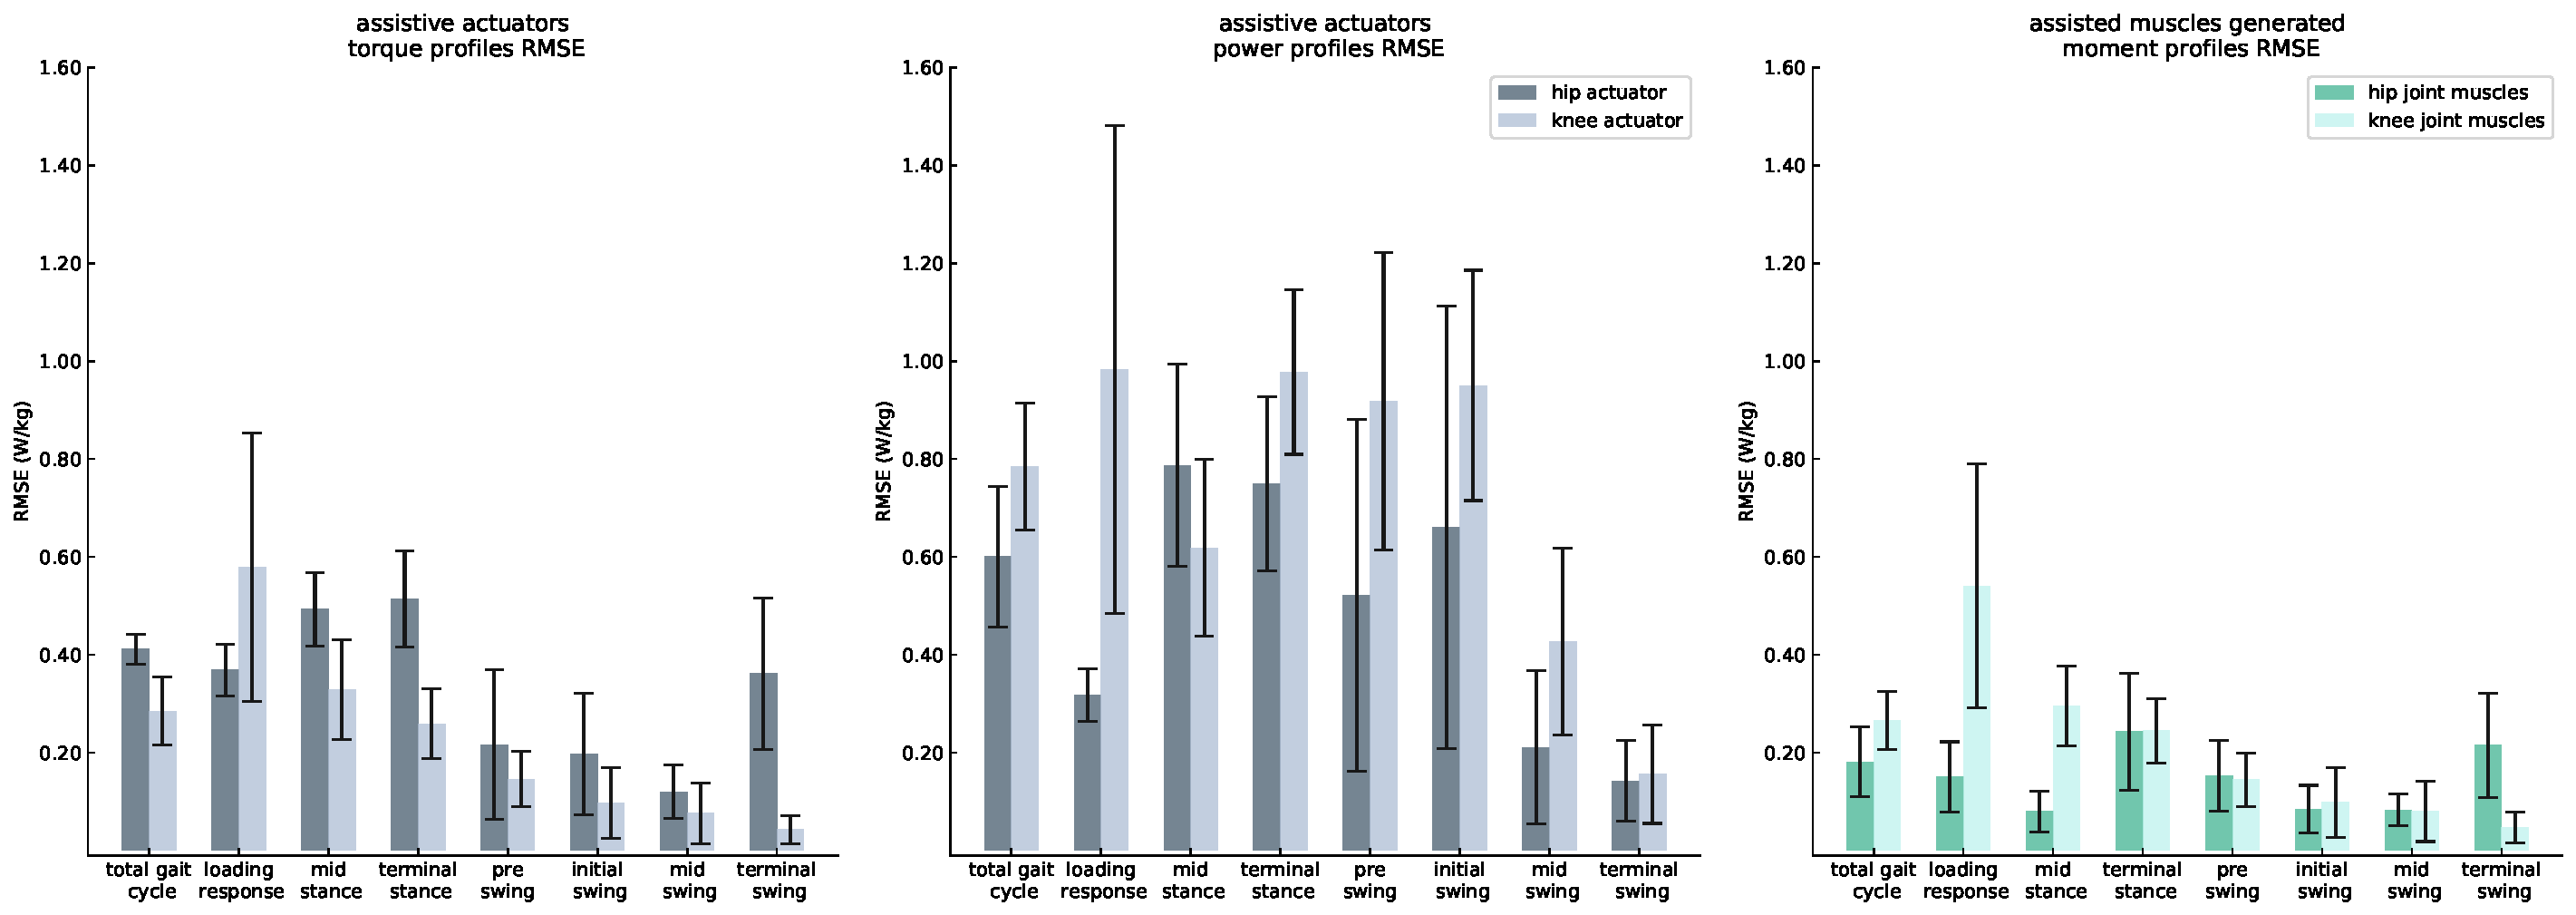
\includegraphics[width=\linewidth]{Case_Studies/LoadedMono04_LoadedBi16/RMSE.pdf}
	\vspace{1mm}
	\caption{\small{\textbf{Assistive devices torque, power, and muscles generated moment profiles root mean square error. } The root mean square error between actuators of biarticular and monoarticular devices and the muscles generated moment of subjects assisted by these devices.}}
	\label{Fig_Case01_RMSE}
\end{figure*}
\begin{figure*}[ht]   
	\centering
	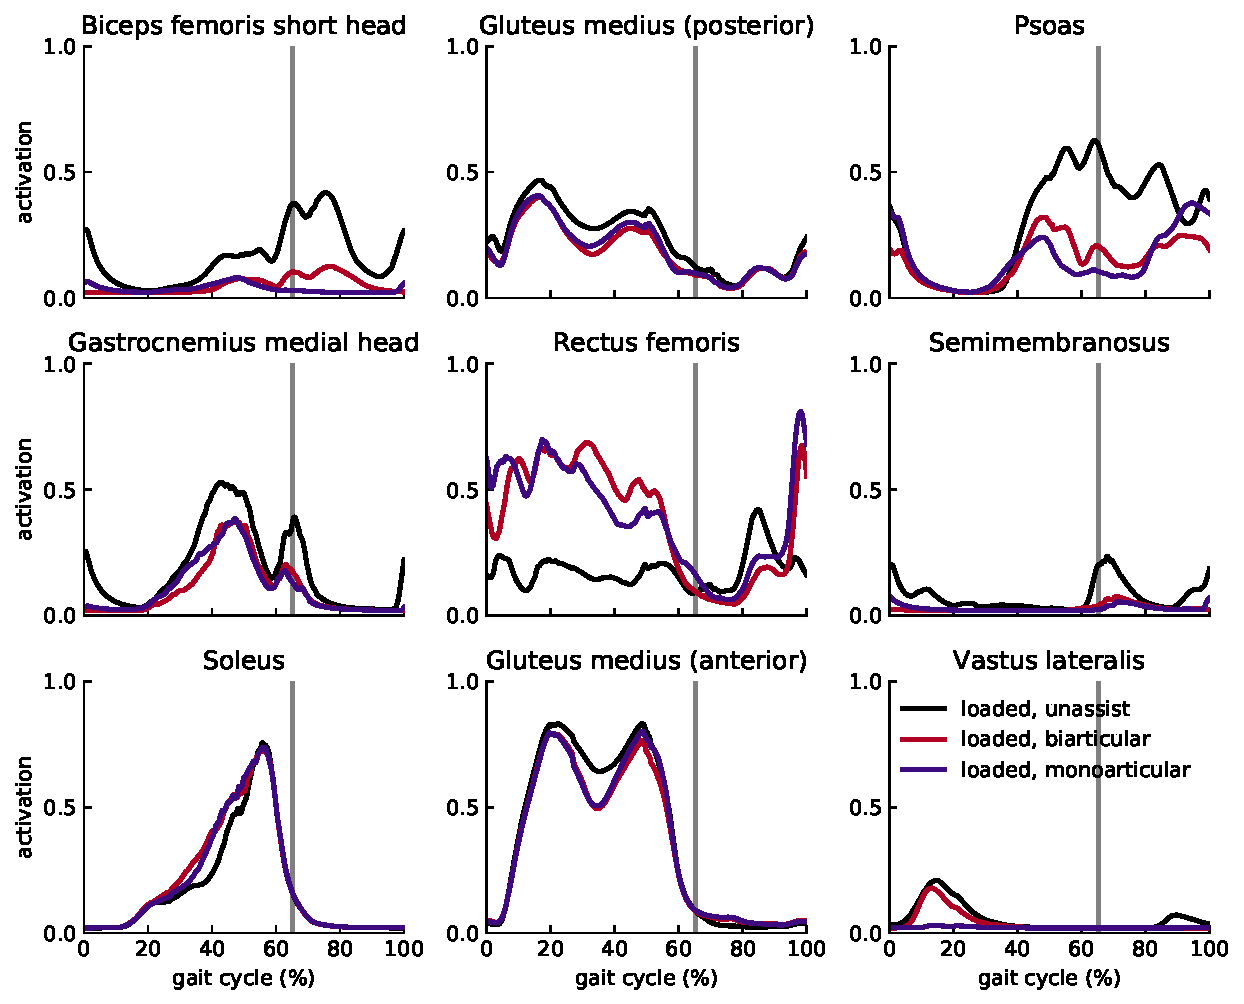
\includegraphics[width=\linewidth]{Case_Studies/LoadedMono04_LoadedBi16/MonoarticularVSBiarticular_Loaded_MusclesActivation.pdf}
	\vspace{1mm}
	\caption{\small{\textbf{Activation of representative lower limb muscles of assisted and unassisted subjects.} The activation of unassisted subjects carrying heavy load (black), and subjects assisted by "Ad" monoarticular (dark purple), and "Da" biarticular (dark pink) devices are shown for nine important muscles. The curves are averaged over 7 subjects with 3 trials.}}
	\label{Fig_Case01_MusclesActivity}
\end{figure*}
The overall trend between torque profiles of the monoarticular and biarticular devices was similar, which can be seen in Figure \ref{Fig_Case01_Torque_Power_Profiles} qualitatively, and the root mean square error between the profiles of the selected devices during a gait cycle also supports this claim quantitatively, as shown in Figure \ref{Fig_Case01_RMSE}. The detailed analysis of the gait cycle shows that the main difference between the torque profiles of the hip actuators occurred during the stance phases, and the monoarticular delivered hip extension torque more than the biarticular device, especially during the mid-stance and terminal-stance phases (Figure \ref{Fig_Case01_Torque_Power_Profiles} and \ref{Fig_Case01_RMSE}). Although the difference between the profiles of the hip actuators followed similar trajectories during the swing phase, the terminal-swing phase of these actuators was considerably different in which the monoarticular delivered extension while biarticular provided flexion torque to the joint.\\
Although the biarticular and monoarticular knee actuators had almost identical trajectories during the swing phase, as their RMSE shows in Figure \ref{Fig_Case01_RMSE}, there were some significant differences between these two actuators during the stance phases. While the biarticular knee actuator opposed with the torque generated by muscles around the knee joint during all stance phase, the monoarticular knee actuator assisted the knee muscles generated torque during the loading response and mid-stance phases.\\
These remarkable differences between torque profiles of two devices affected the torque trajectories generated by muscles around the knee and hip joints, indicating muscular activation differences between subjects assisted by the monoarticular and biarticular exoskeletons; nevertheless, according to the root mean square error between hip and knee muscles generated torque trajectories, the differences were not substantial except on the loading phase of the knee joint.\\
The comparison between the muscular activation of the {\it loaded} subjects assisted by ideal devices and constrained devices indicates substantial differences in some muscles. The activation of rectus femoris and psoas as two primary muscles on the hip and knee were considerably different in the ideal and constrained devices.  The constrained biarticular and monoarticular exoskeletons also had different impacts on these two muscles ( Figure \ref{Fig_Case01_MusclesActivity}). The difference between the activation of rectus femoris and vasti muscles of subjects assisted by the constrained optimal biarticular and monoarticular devices during the loading response phase can explain the difference between the muscles generated moments of subjects assisted by the biarticular and monoarticular devices. Another remarkable difference between the ideal and constrained devices was in gastrocnemius medial head muscle, in which the activation of this muscle increased during the loading response to terminal stance phases. Due to the higher activation of the gastrocnemius muscle, it provided more moment on the ankle joint. Consequently, the activation of the soleus muscle did not increase considerably to compensate for the inadequacy of the moment generated by gastrocnemius at the ankle joint.
The differences between the muscular activation of subjects assisted by monoarticular and biarticular constrained devices were not limited to the rectus femoris and psoas muscles, but the other representative muscles demonstrated some differences, as shown in the Figure \ref{Fig_Case01_MusclesActivity}, nevertheless, the differences between them were not as considerable as rectus femoris and psoas muscles.\\
Unlike the moment profiles of devices in which the difference was significant only in some specific phases, the power profiles of the biarticular and monoarticular devices had significant differences, as shown qualitatively and quantitatively in Figures \ref{Fig_Case01_Torque_Power_Profiles} and \ref{Fig_Case01_RMSE} respectively. The difference between the power profiles of these two devices was remarkable in the knee actuator in which the devices followed different trajectories during the gait cycle. Similar to the knee actuators, the hip actuators also had roughly different power profiles, and their maximum power consumption occurred in two completely different phases, similar to the knee actuators.  The difference between the trajectories and magnitudes of the power profiles also can explain the statistically significant difference observed between the monoarticular and biarticular exoskeletons (Fig.\ref{Fig_Case01_Energy_Plot}).\\
Studying the selected monoarticular and biarticular devices proves the devices with the same total power consumption can have different power consumption in different joints. Additionally, we showed that the optimal devices with the same performance can follow different moment and power profiles, even under kinematic similarities due to the arrangement of actuators. Although the devices were selected from the ideal Pareto front with the same performance, employing the modified augmentation factor for the monoarticular and biarticular devices with different mass and inertia characteristics indicated the superior performance of the biarticular device. It emphasizes the discussion held in the "Effect of Optimal Device Inertial Properties on Subject Metabolics" section in that the biarticular device could deliver the same amount of assistance to the subjects more effectively than the monoarticular configuration.\\
%%%%%%%%%%%%%%%%%%%%%%%%%%%%%%%%%%%%%%%%%%%%%%%%%%%%%%%%%%%%%%%%%%%%%%%%%%%%%%%%%%%%%%%%%%%%%%%%%%%%%%%%%%%%%%%%%%%%%
\section*{Case 2: Devices Performance in \textit{\textit{noload}} Condition}
In the second case study, we selected two devices with almost similar power consumptions and the same effect on the metabolic rate of subjects walking without any extra load, which are shown as "Cb" and "Ba" on the Pareto front curves of the biarticular and monoarticular devices in the {\it noload} condition, respectively. Although the total performance of these two biarticular and monoarticular devices were different in mean values on the trade-off curves, the statistical tests on the absolute power consumption of actuator showed no statistically significant difference between actuators of the monoarticular and biarticular exoskeletons.\\
\begin{figure*}[ht]   
	\centering
	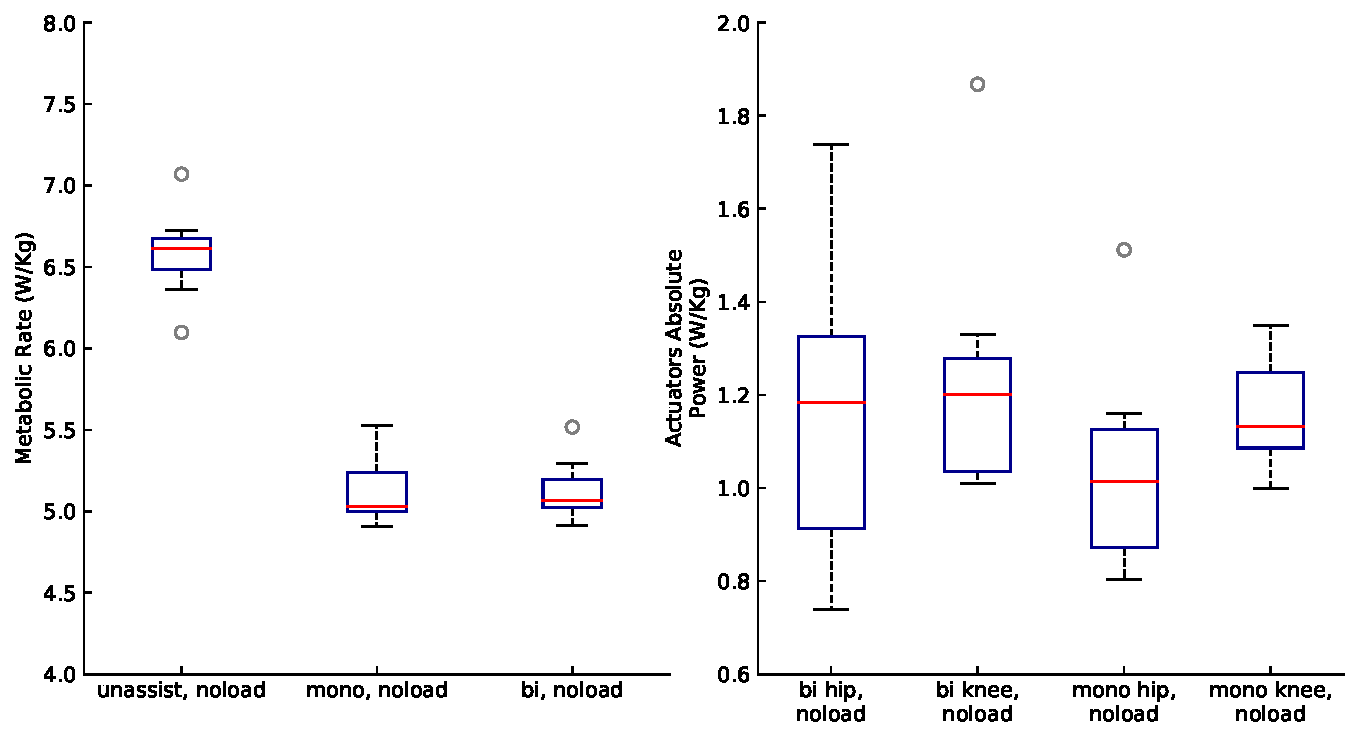
\includegraphics[width=\linewidth]{Case_Studies/NoloadMono06_NoloadBi12/PaperFigure_BoxPlot.pdf}
	\vspace{1mm}
	\caption{\small{\textbf{Assistive devices power consumption and its effect on the metabolic rate.} The power consumptions of assistive devices and their effect on whole-body metabolic rate of the subjects walking at self-selected speed without any additional load. Asterisks indicate statistically significant differences ( 7 subjects, 3 trails, Tukey Post-hoc, $P < 0.05$).}}
	\label{Fig_Case02_Energy_Plot}
\end{figure*}
\begin{figure*}[ht]   
	\centering
	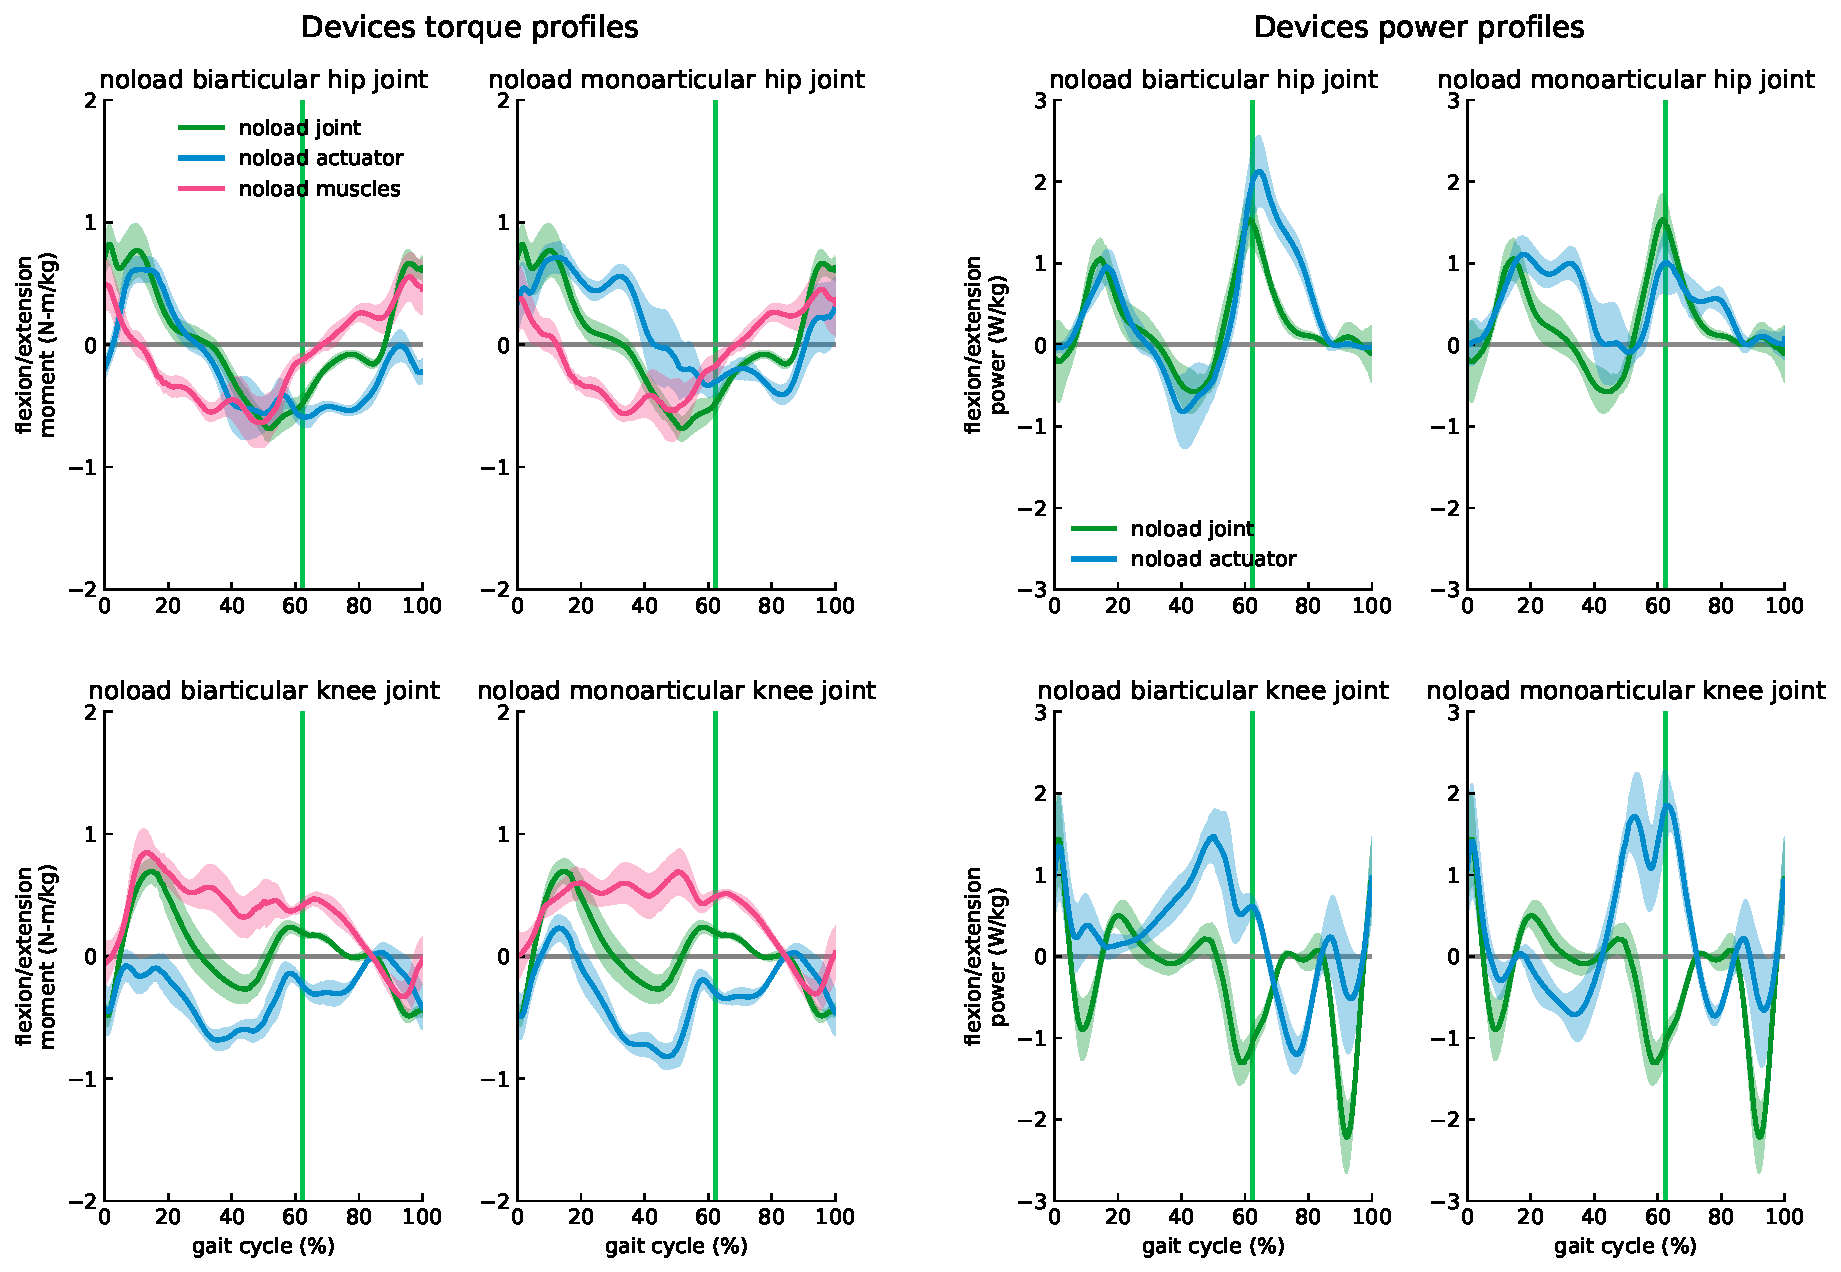
\includegraphics[width=\linewidth]{Case_Studies/NoloadMono06_NoloadBi12/PaperFigure_Profiles.pdf}
	\vspace{1mm}
	\caption{{\small\textbf{Assistive devices torque and power profiles.} The actuator torque and power for subjects walking without an additional load (blue) , and net joint power and torque profile for \textit{noload} (green) condition are shown for each actuator of the devices. The torque profile of moment generated by muscles (rose pink) is shown for each joint for both devices. The curves are averaged over 7 subjects with 3 trials and normalized by subject mass; shaded regions around the mean profile indicate standard deviation of the profile.}}
	\label{Fig_Case02_Torque_Power_Profiles}
\end{figure*}
\begin{figure*}[ht]   
	\centering
	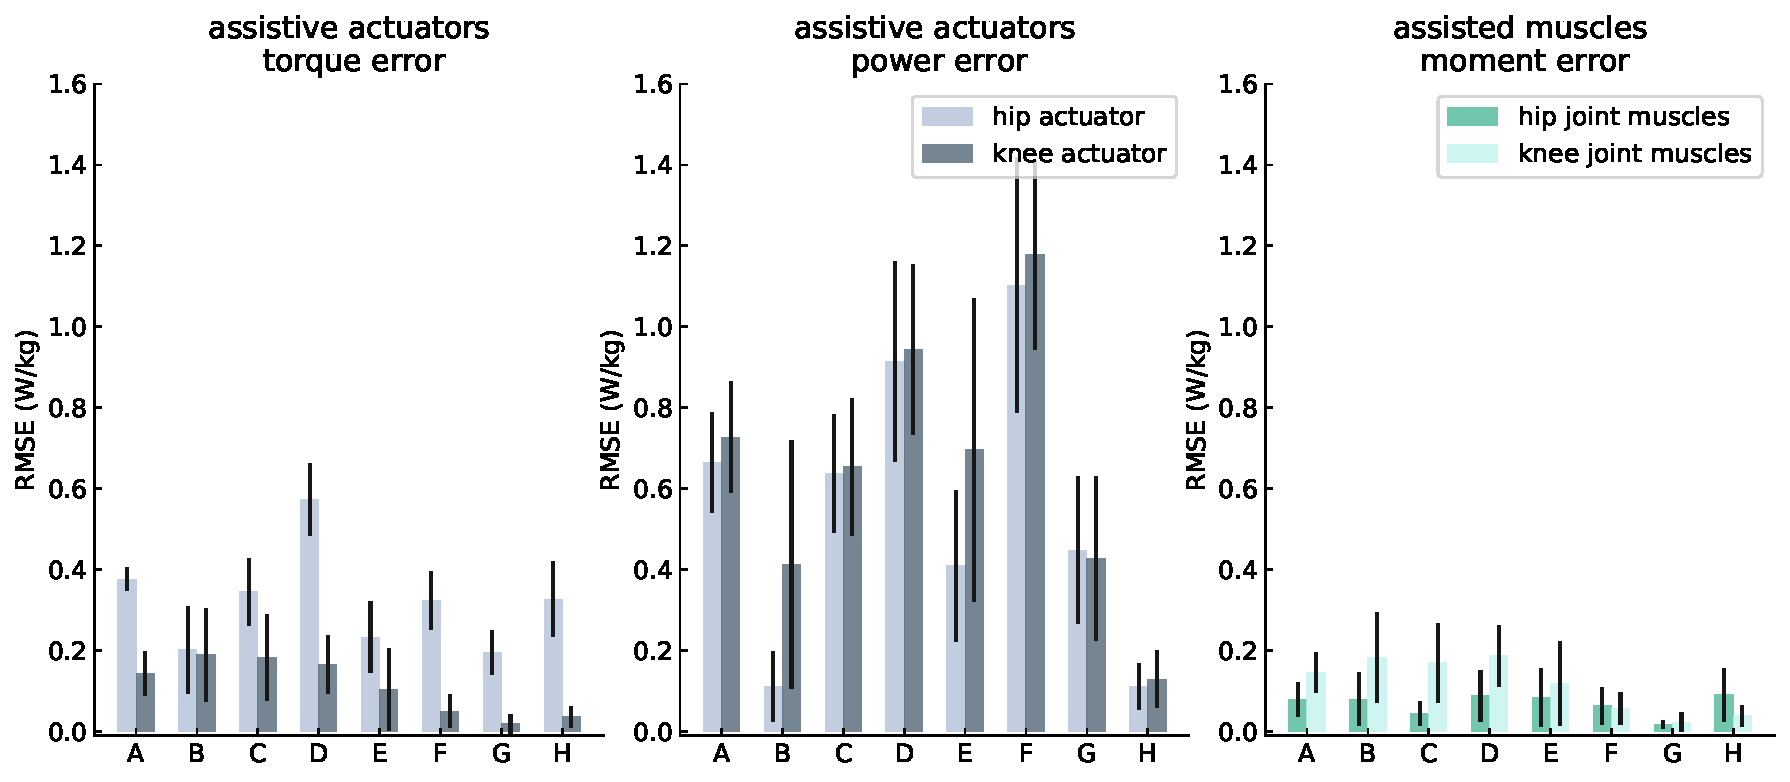
\includegraphics[width=\linewidth]{Case_Studies/NoloadMono06_NoloadBi12/RMSE.pdf}
	\vspace{1mm}
	\caption{\small{\textbf{Assistive devices torque, power, and muscles generated moment profiles root mean square error. } The root mean square error between actuators of biarticular and monoarticular devices and the muscles generated moment of subjects assisted by these devices.}}
	\label{Fig_Case02_RMSE}
\end{figure*} 
The power consumption of the hip actuators in both exoskeletons had a high within-subject deviation, as shown in Figure \ref{Fig_Case02_Energy_Plot}, which can explain the absence of statistically significant differences between the actuators.  Additionally, the metabolic rate of subjects assisted with the monoarticular and biarticular devices had no significant differences. However, the metabolic cost reduction caused a significant difference between the metabolic expenditure of unassisted and assisted subjects, as represented in Figure \ref{Fig_Case02_Energy_Plot}.
Despite the large variation between the power consumption of the devices and the absence of significant difference among their actuators, employing the modified augmentation factor indicates remarkably different performance of the monoarticular and biarticular exoskeletons delivering assistance to the subjects. The selected devices had a different design in the actuators in which the biarticular device could provide maximum 50 and 60 N-m torque in the hip and knee actuators, respectively, while the maximum moments in the hip and knee actuators of the monoarticular device were 60 and 70 N-m, respectively. The computation of MAF under mentioned configurations of these two devices resulted in 1.57$\pm$0.72 and 0.42$\pm$0.85 W/kg for the biarticular and monoarticular devices, respectively, indicating the superior performance of the biarticular device similar to the first case. The performance of these two devices can also be discussed based on the Pareto front of devices under inertia and mass effect shown in Figure 17 in the paper. According to this analysis, the studied configuration of the monoarticular device became a dominated solution in Pareto simulations under the inertial properties of devices, while the chosen biarticular device could maintain its efficiency under the negative effect of its inertial properties on the metabolic rate of subjects. This analogy between the Pareto front with devices inertial properties effect consideration and MAF can also confirm the extension of the augmentation factor.\\
The analysis of moment profiles of assistive devices in the {\it noload} condition shows that the differences between these two devices were similar to the difference of biarticular and monoarticular devices in the {\it loaded} circumstance, which is represented in Figure \ref{Fig_Case02_Torque_Power_Profiles}. Nevertheless, the variations of moment generated by muscles of the assisted subjects were negligible in {\it noload} condition (Figure \ref{Fig_Case02_RMSE}), which signals similar muscular activation of subjects assisted with these two exoskeletons. Unlike the moment profiles, the power profiles of the devices were different in the {\it noload} condition. It can be seen from the power profiles that the devices followed remarkably different trajectories during a gait cycle to deliver assistance to the subjects and these profiles in the hip actuators, similar to the knee actuators, had the highest contrast during the pre-swing phase according to their RMS error, as shown in Figure \ref{Fig_Case02_RMSE}.\\
Studying specific optimal monoarticular and biarticular exoskeletons in two load conditions, chosen from the Pareto fronts, shows that even though the devices had practically the same performance in the optimal trade-off between the device total power consumption and metabolic cost reduction curves, their provided moment during a gait cycle had considerable differences, which could cause a different effect on the muscular activation of assisted subjects as well. These two case studies also show that the power profiles of monoarticular and biarticular devices are considerably different, while they have a similar total power consumption.\\
The study on the performance of selected devices in both loading conditions by developed MAF factor supports the discussion held on the "Effect of Optimal Device Inertial Properties on Subject Metabolics" section on the effect of the mechanical design on the performance of devices and also showed that the performance of the monoarticular exoskeleton was highly affected by the inertial properties of the device. Although the mechanical design of a biarticular device can be complicated, its performance under the device inertial properties seems promising in both loading conditions according to the performance of studied cases. The studied cases and general Pareto front of monoarticular device under its inertial characteristics effect show that the monoarticular device needs to be designed thoughtfully to reduce the effect of inertia and mass effect of the device on the metabolic burden of subjects complicating the design procedure, and ignoring the mechanical design results in delivering no assistance to the subject, or increasing their metabolic burden. 
%%%%%%%%%%%%%%%%%%%%%%%%%%%%%%%%%%%%%%%%%%%%%%%%%%%%%%%%%%%%%%%%%%%%%%%%%%%%%%%%%%%%%%%%%%%%%%%%%%%%%%%%%%%%%%%%%%%%
\section*{Case 3: Biarticular Exoskeleton Performance}
To study how the performance of a biarticular exoskeleton changes by loading subjects with a heavy weight on torso more specifically, we chose two cases in which the biarticular exoskeletons had the same effect on the metabolic rate of subjects in one case, and they had the same power consumption in another case.\\ 
\begin{figure*}[th!]
	\centering
	\subfloat[\small{Biarticular exoskeleton with the same effect on the metabolic consumption of subjects}]{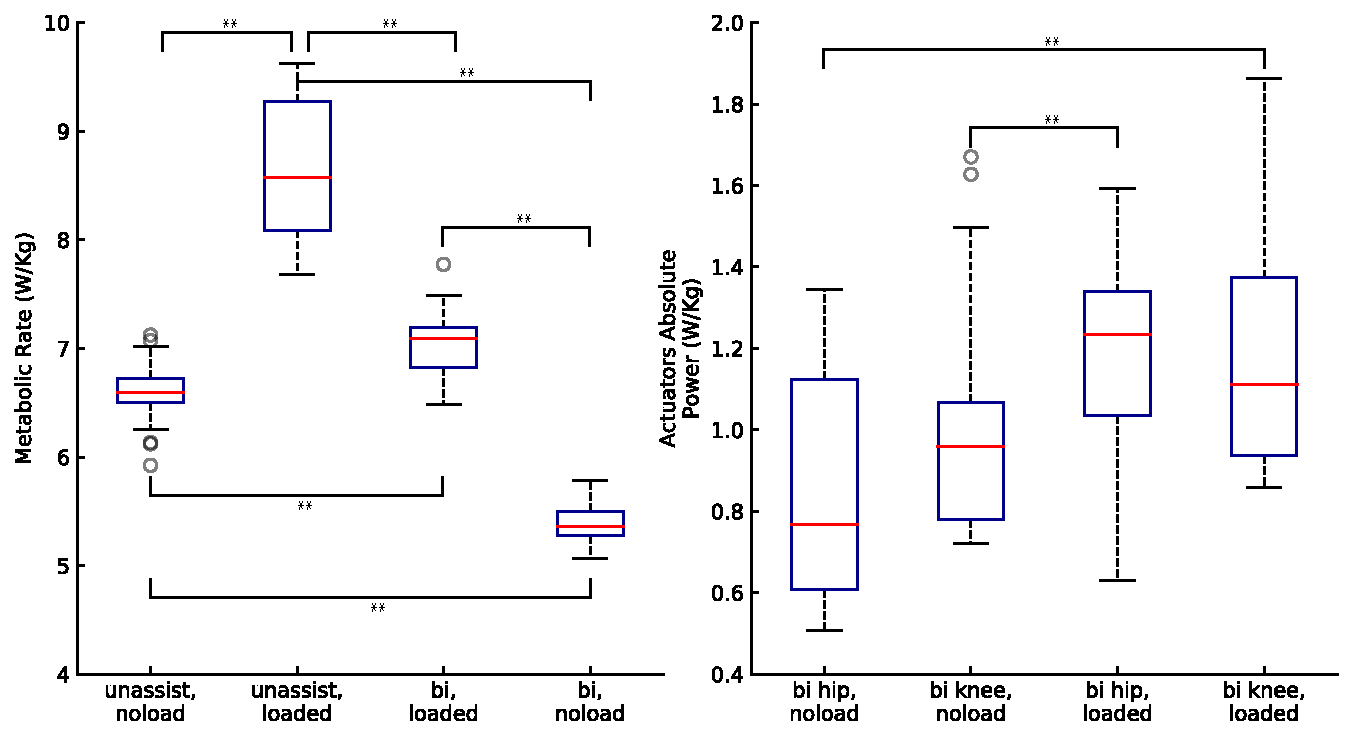
\includegraphics[width=\linewidth]{Case_Studies/NoloadBi23_LoadedBi12/PaperFigure_BoxPlot.pdf}
		\label{Fig_Case03_Energy_Plot_SameMetabolicConsumption}}
	\hfil
	\subfloat[\small{Biarticular exoskeleton with the same total power consumptions }]{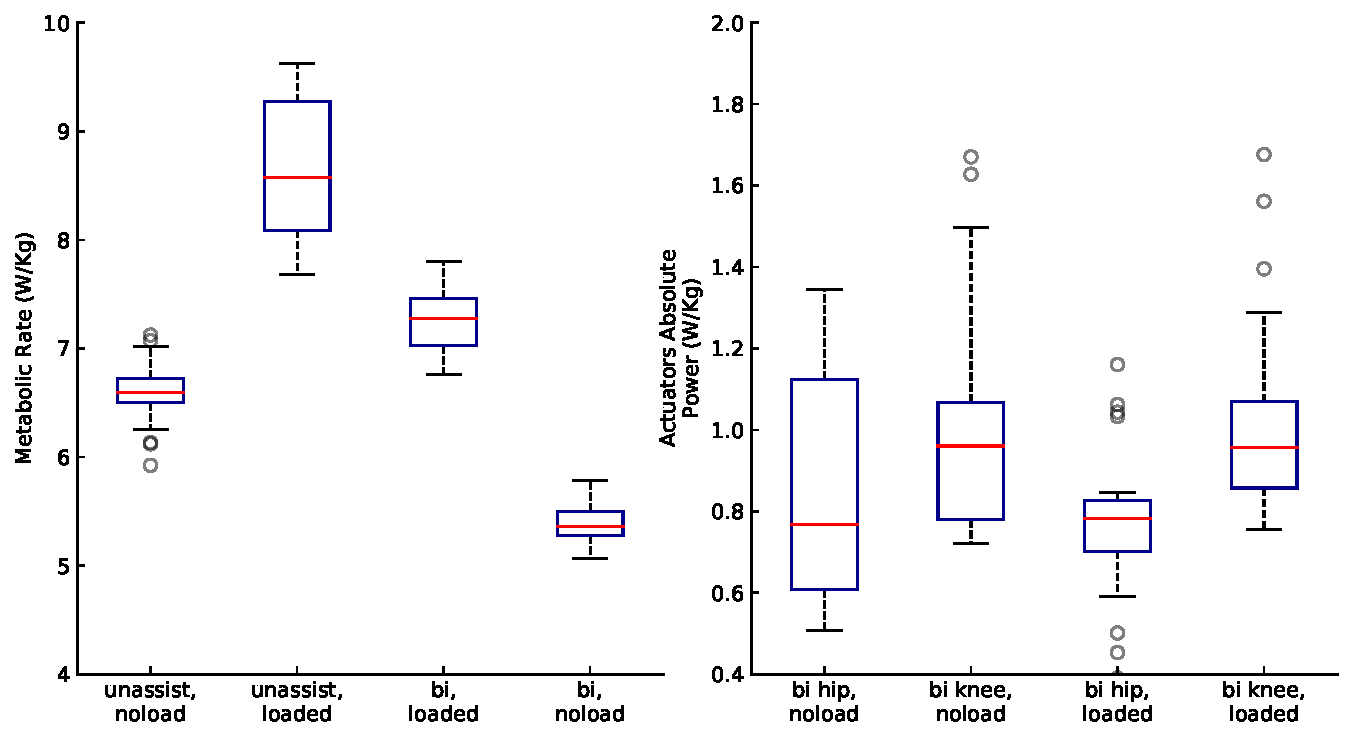
\includegraphics[width=\linewidth]{Case_Studies/NoloadBi23_LoadedBi23/PaperFigure_BoxPlot.pdf}
		\label{Fig_Case03_Energy_Plot_SamePowerConsumption}}
	\vspace{2mm}
	\caption{\small{\textbf{Biarticular exoskeleton power consumption and its effect on the metabolic rate in different load conditions.} The power consumptions of biarticular exoskeleton and their effect on whole-body metabolic rate of the subjects walking at self-selected speed in both {\it loaded} and {\it noload} condition. Asterisks indicate statistically significant differences ( 7 subjects, 3 trails, Tukey Post-hoc, $P < 0.05$).}}
	\label{Fig_Case03_Energy_Plot}
\end{figure*}
\begin{figure*}[ht!]
	\centering
	\subfloat[\small{Biarticular exoskeleton with the same effect on the metabolic consumption of subjects}]{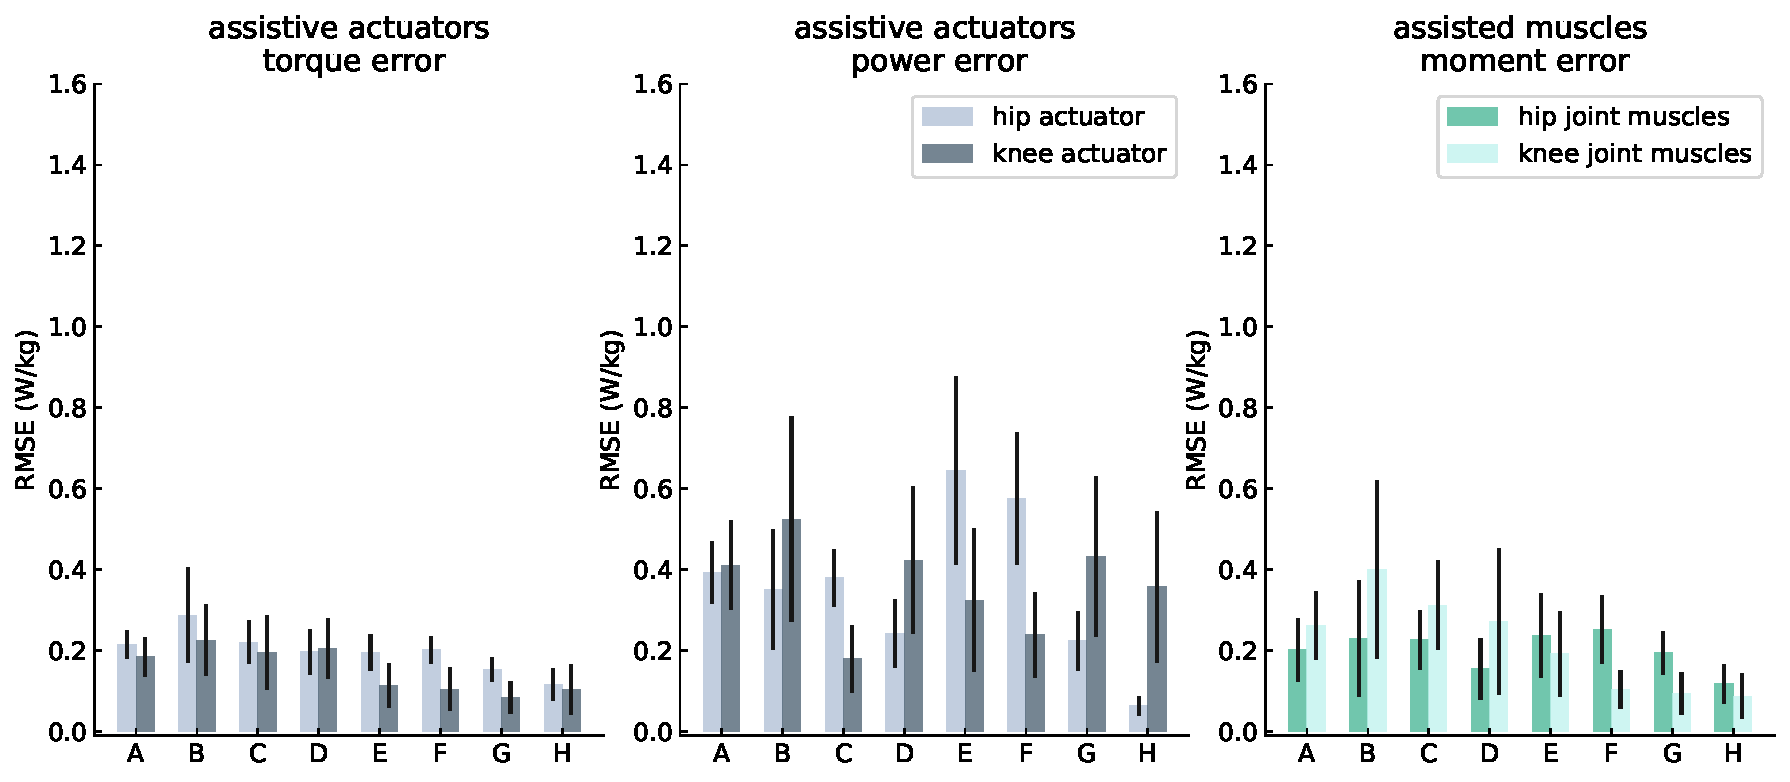
\includegraphics[width=\linewidth]{Case_Studies/NoloadBi23_LoadedBi12/RMSE.pdf}
		\label{Fig_Case03_RMSE_SameMetabolicConsumption}}
	\hfil
	\subfloat[\small{Biarticular exoskeleton with the same total power consumptions }]{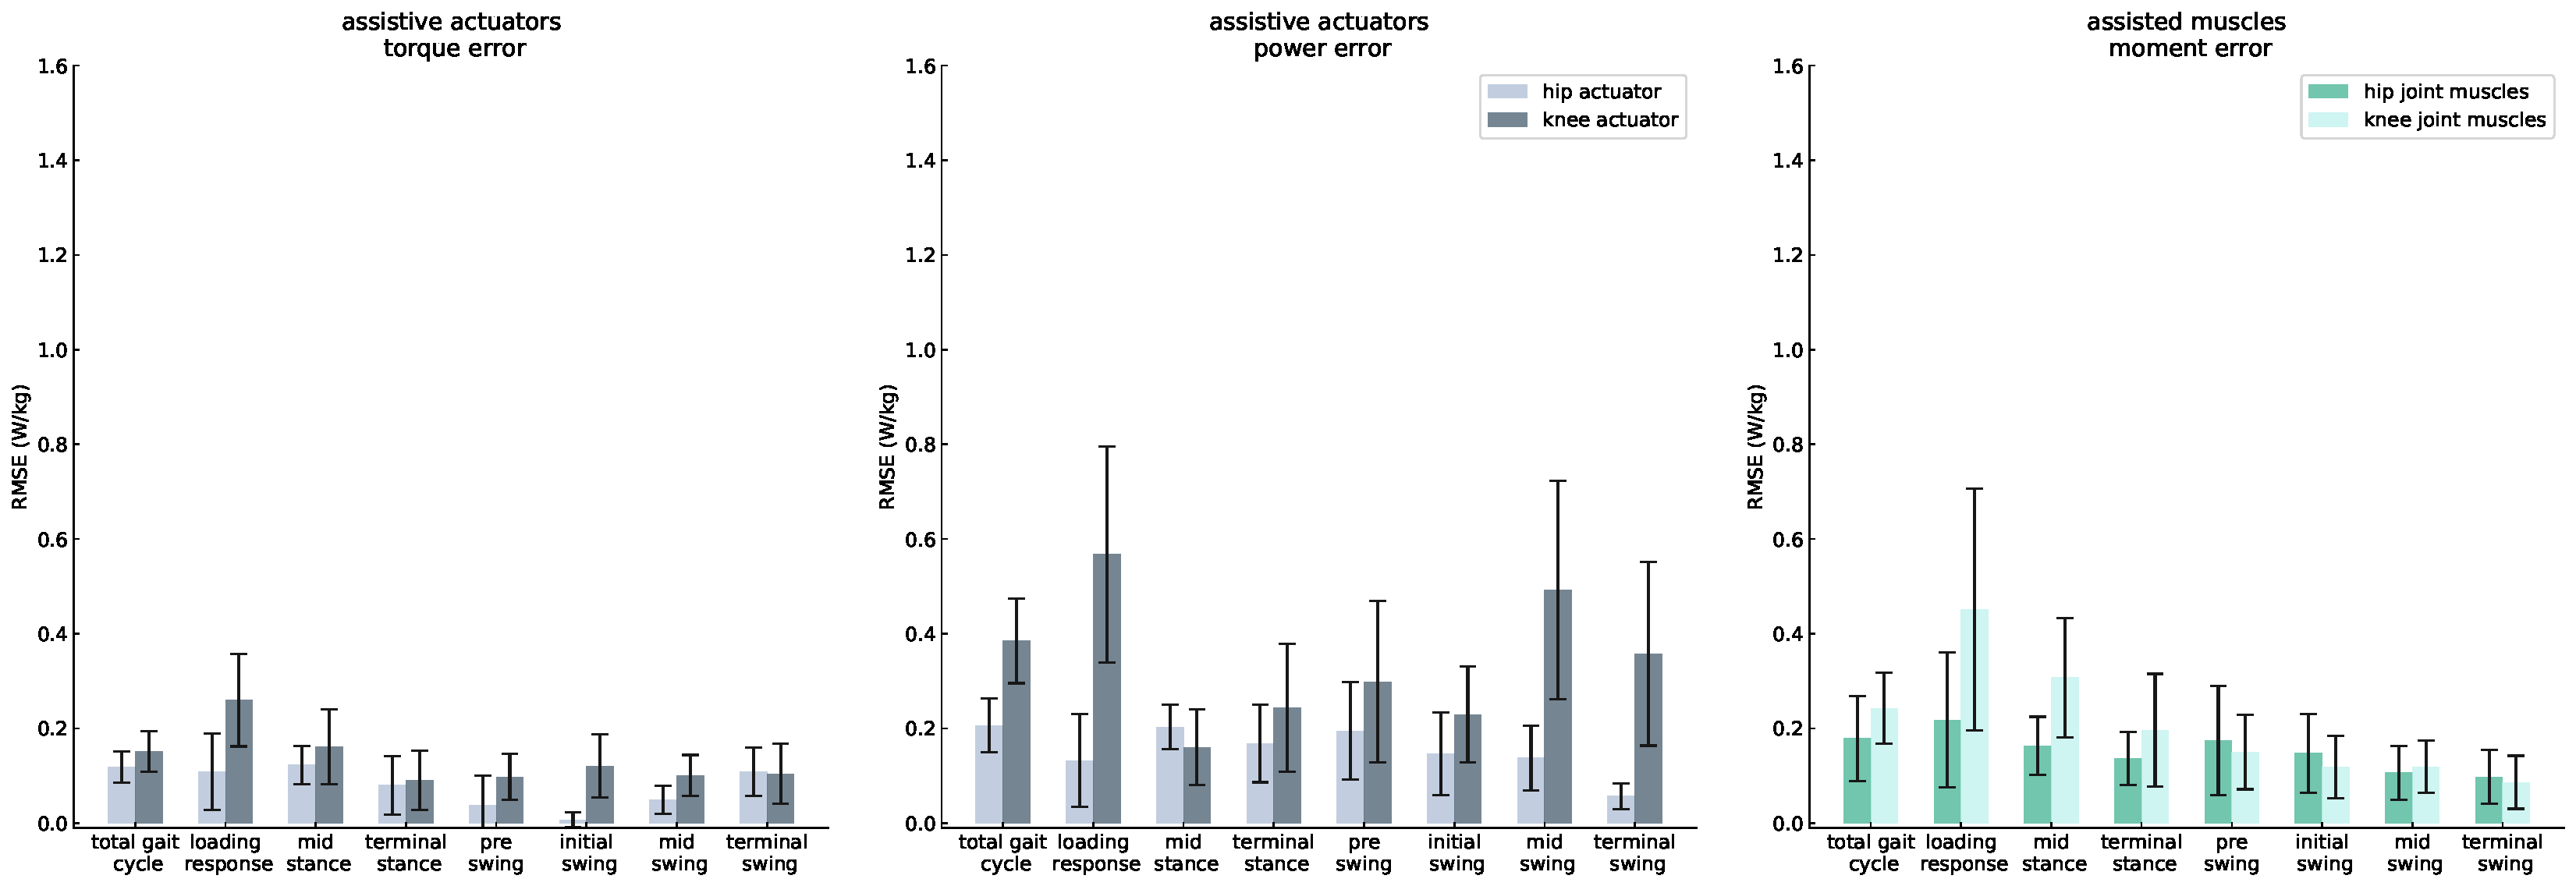
\includegraphics[width=\linewidth]{Case_Studies/NoloadBi23_LoadedBi23/RMSE.pdf}
		\label{Fig_Case03_RMSE_SamePowerConsumption}}
	\vspace{1mm}
	\caption{\small{\textbf{Biarticular exoskeleton torque and power and muscles generated moment profiles root mean square error in different load conditions.} The root mean square error between actuators of the biarticular exoskeleton and the muscles generated moment of subjects assisted by this device {\it loaded} and {\it noload} conditions.}}
	\label{Fig_Case03_RMSE}
\end{figure*}
The selected configuration of the biarticular exoskeleton in {\it noload} condition was "Ec" with 30 and 50 N-m peak torque in the hip and knee actuators, and it was compared to the same configuration (i.e., "Ec") in the {\it loaded} condition in which they had practically the same power consumption. In order to conduct the comparison with the similar metabolic burden reduction, the same configuration of the device in the {\it noload} condition (i.e., "Ec") was compared to the biarticular exoskeleton with 50 and 60 N-m peak torque in the hip and knee actuators represented by "Cb" on the Pareto front of the {\it loaded} biarticular exoskeleton.\\
Comparing the metabolic rate of assisted subjects by the biarticular devices in two conditions, which were similar metabolic cost reduction condition and the same power consumption condition, were represented in Figure \ref{Fig_Case03_Energy_Plot}. The metabolic rates of subjects in both conditions show that even though the metabolic rate of loaded subjects was reduced considerably, there was a statistically significant difference between subjects walking normally and the {\it loaded} subjects assisted by the biarticular device. The power consumption of the hip actuators and knee actuators showed no significant differences when the selected device was consuming a similar amount of power in different loading conditions. Nevertheless, we observed a significant difference between the knee and hip actuators in different load conditions, as shown in Figure \ref{Fig_Case03_RMSE}\subref{Fig_Case03_RMSE_SamePowerConsumption}. Additionally, a similar performance in power consumption of two different configurations of the biarticular exoskeleton delivering a similar amount of assistance in different load conditions has been observed, which is represented in Figure \ref{Fig_Case03_RMSE}\subref{Fig_Case03_RMSE_SameMetabolicConsumption}.\\
The absence of a significant difference between two devices with different configurations and different load conditions can facilitate designing a battery with a robust performance in different load conditions. This performance can also help to have a general mechanical design for an exoskeleton to assist subjects in different load conditions and assistance levels. Nevertheless, the high within-subject deviations and outliers of power consumption indicate high contrast within subjects which can complicate obtaining general power profiles for the device.\\
The performance assessment of the same biarticular configuration in two different load conditions by employing MAF showed that the performance of the biarticular exoskeleton in the {\it loaded} condition was improved (1.40$\pm$0.80 W/kg) in comparison with the  {\it noload} condition, in which the MAF value was 1.01$\pm$0.70 W/kg. Although the increase in the positive power of the device in the {\it loaded} condition was expected, improvement of the MAF value shows that this increase in positive power was delivered to the subjects effectively. In the meanwhile, comparing the devices with the same effect on the metabolic cost reduction of subjects in different load conditions showed superior performance of the biarticular device in the {\it loaded} in which devices in the {\it loaded} and {\it noload} circumstances had  2.08$\pm$0.69 and 1.01 $\pm$0.69 W/kg MAF value, which can indicate inefficiency of noload device power profiles in general.\\
\begin{figure*}[ht!]
	\centering
	\subfloat[\small{Biarticular exoskeleton with the same effect on the metabolic consumption of subjects}]{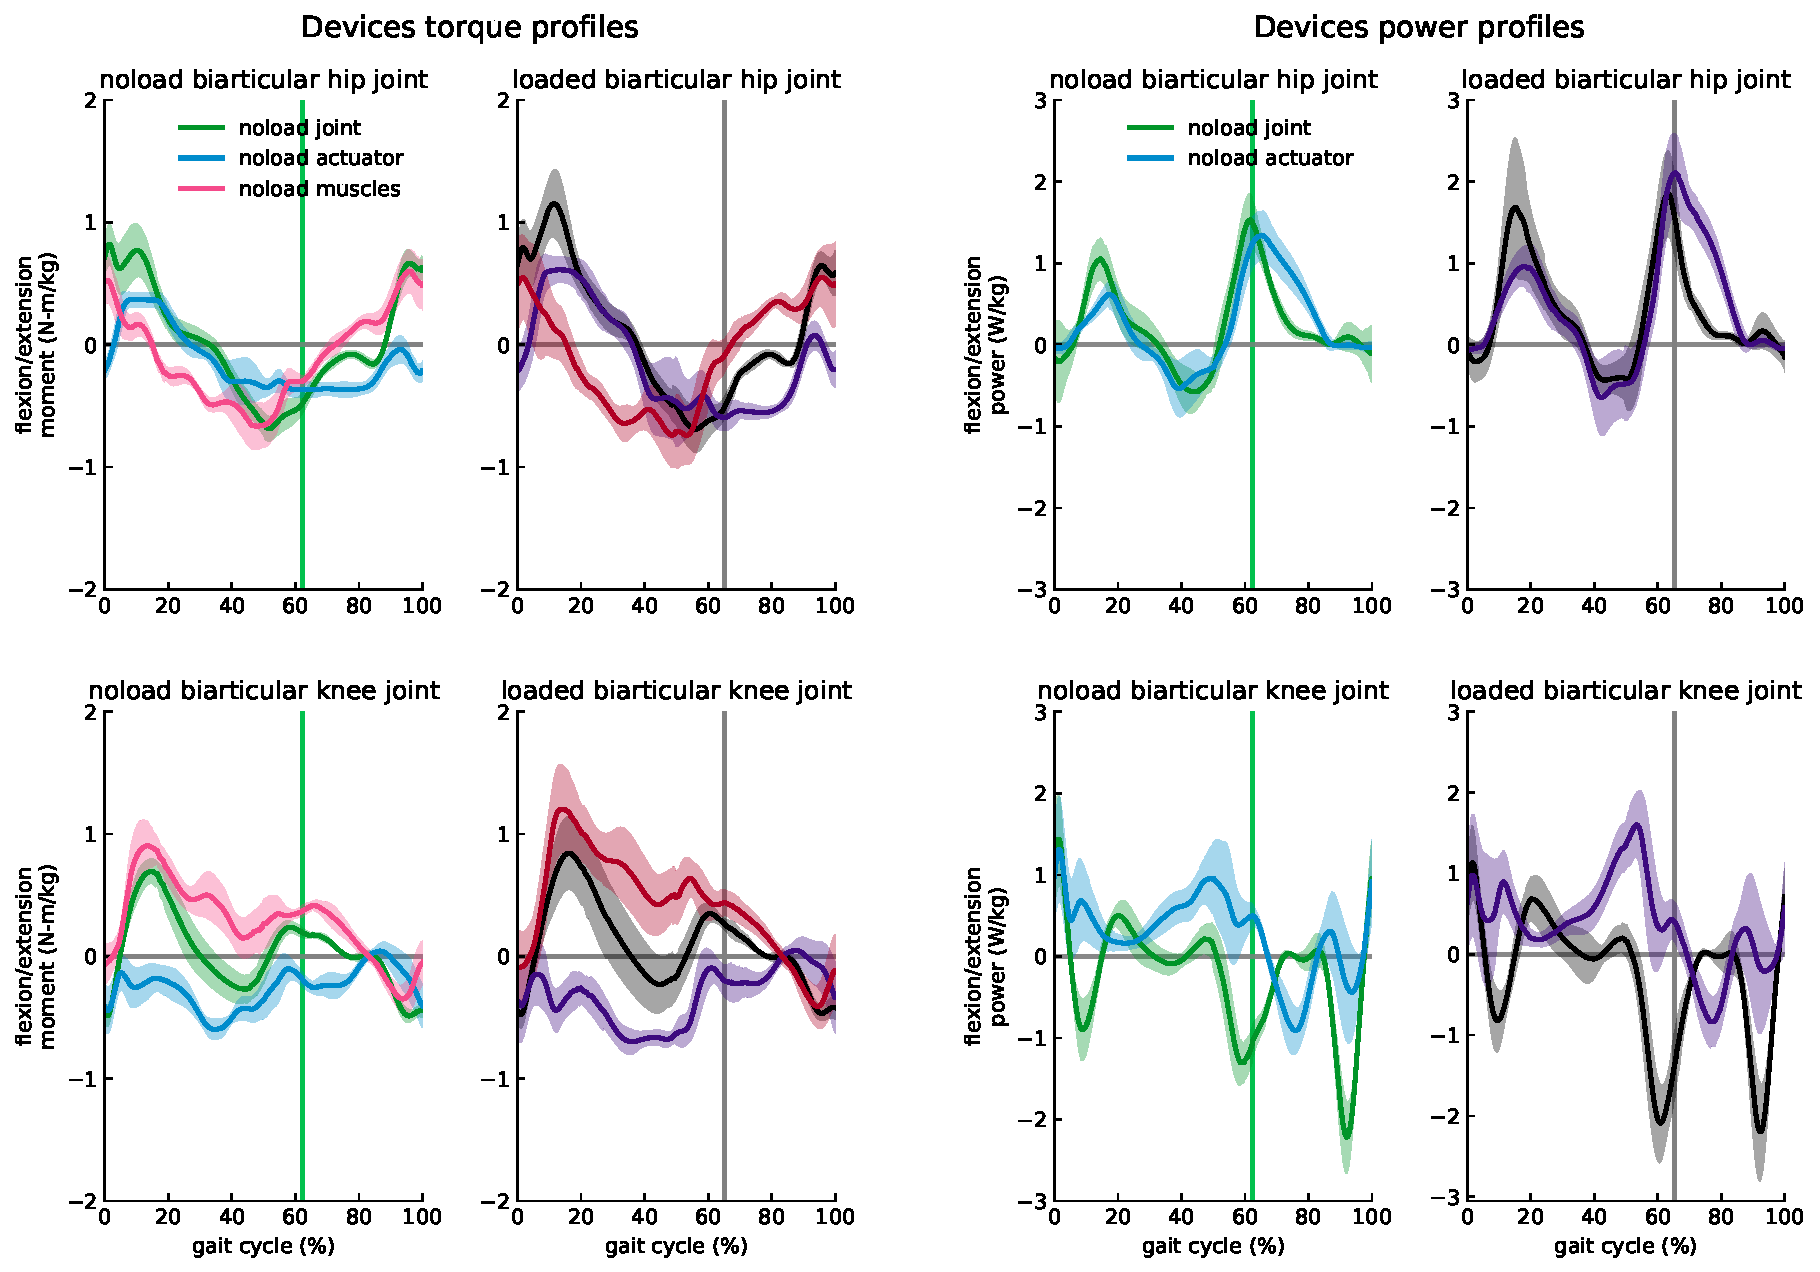
\includegraphics[width=\linewidth]{Case_Studies/NoloadBi23_LoadedBi12/PaperFigure_Profiles.pdf}
		\label{Fig_Case03_SameMetabolicConsumption}}
	\hfil
	\subfloat[\small{Biarticular exoskeleton with the same total power consumptions }]{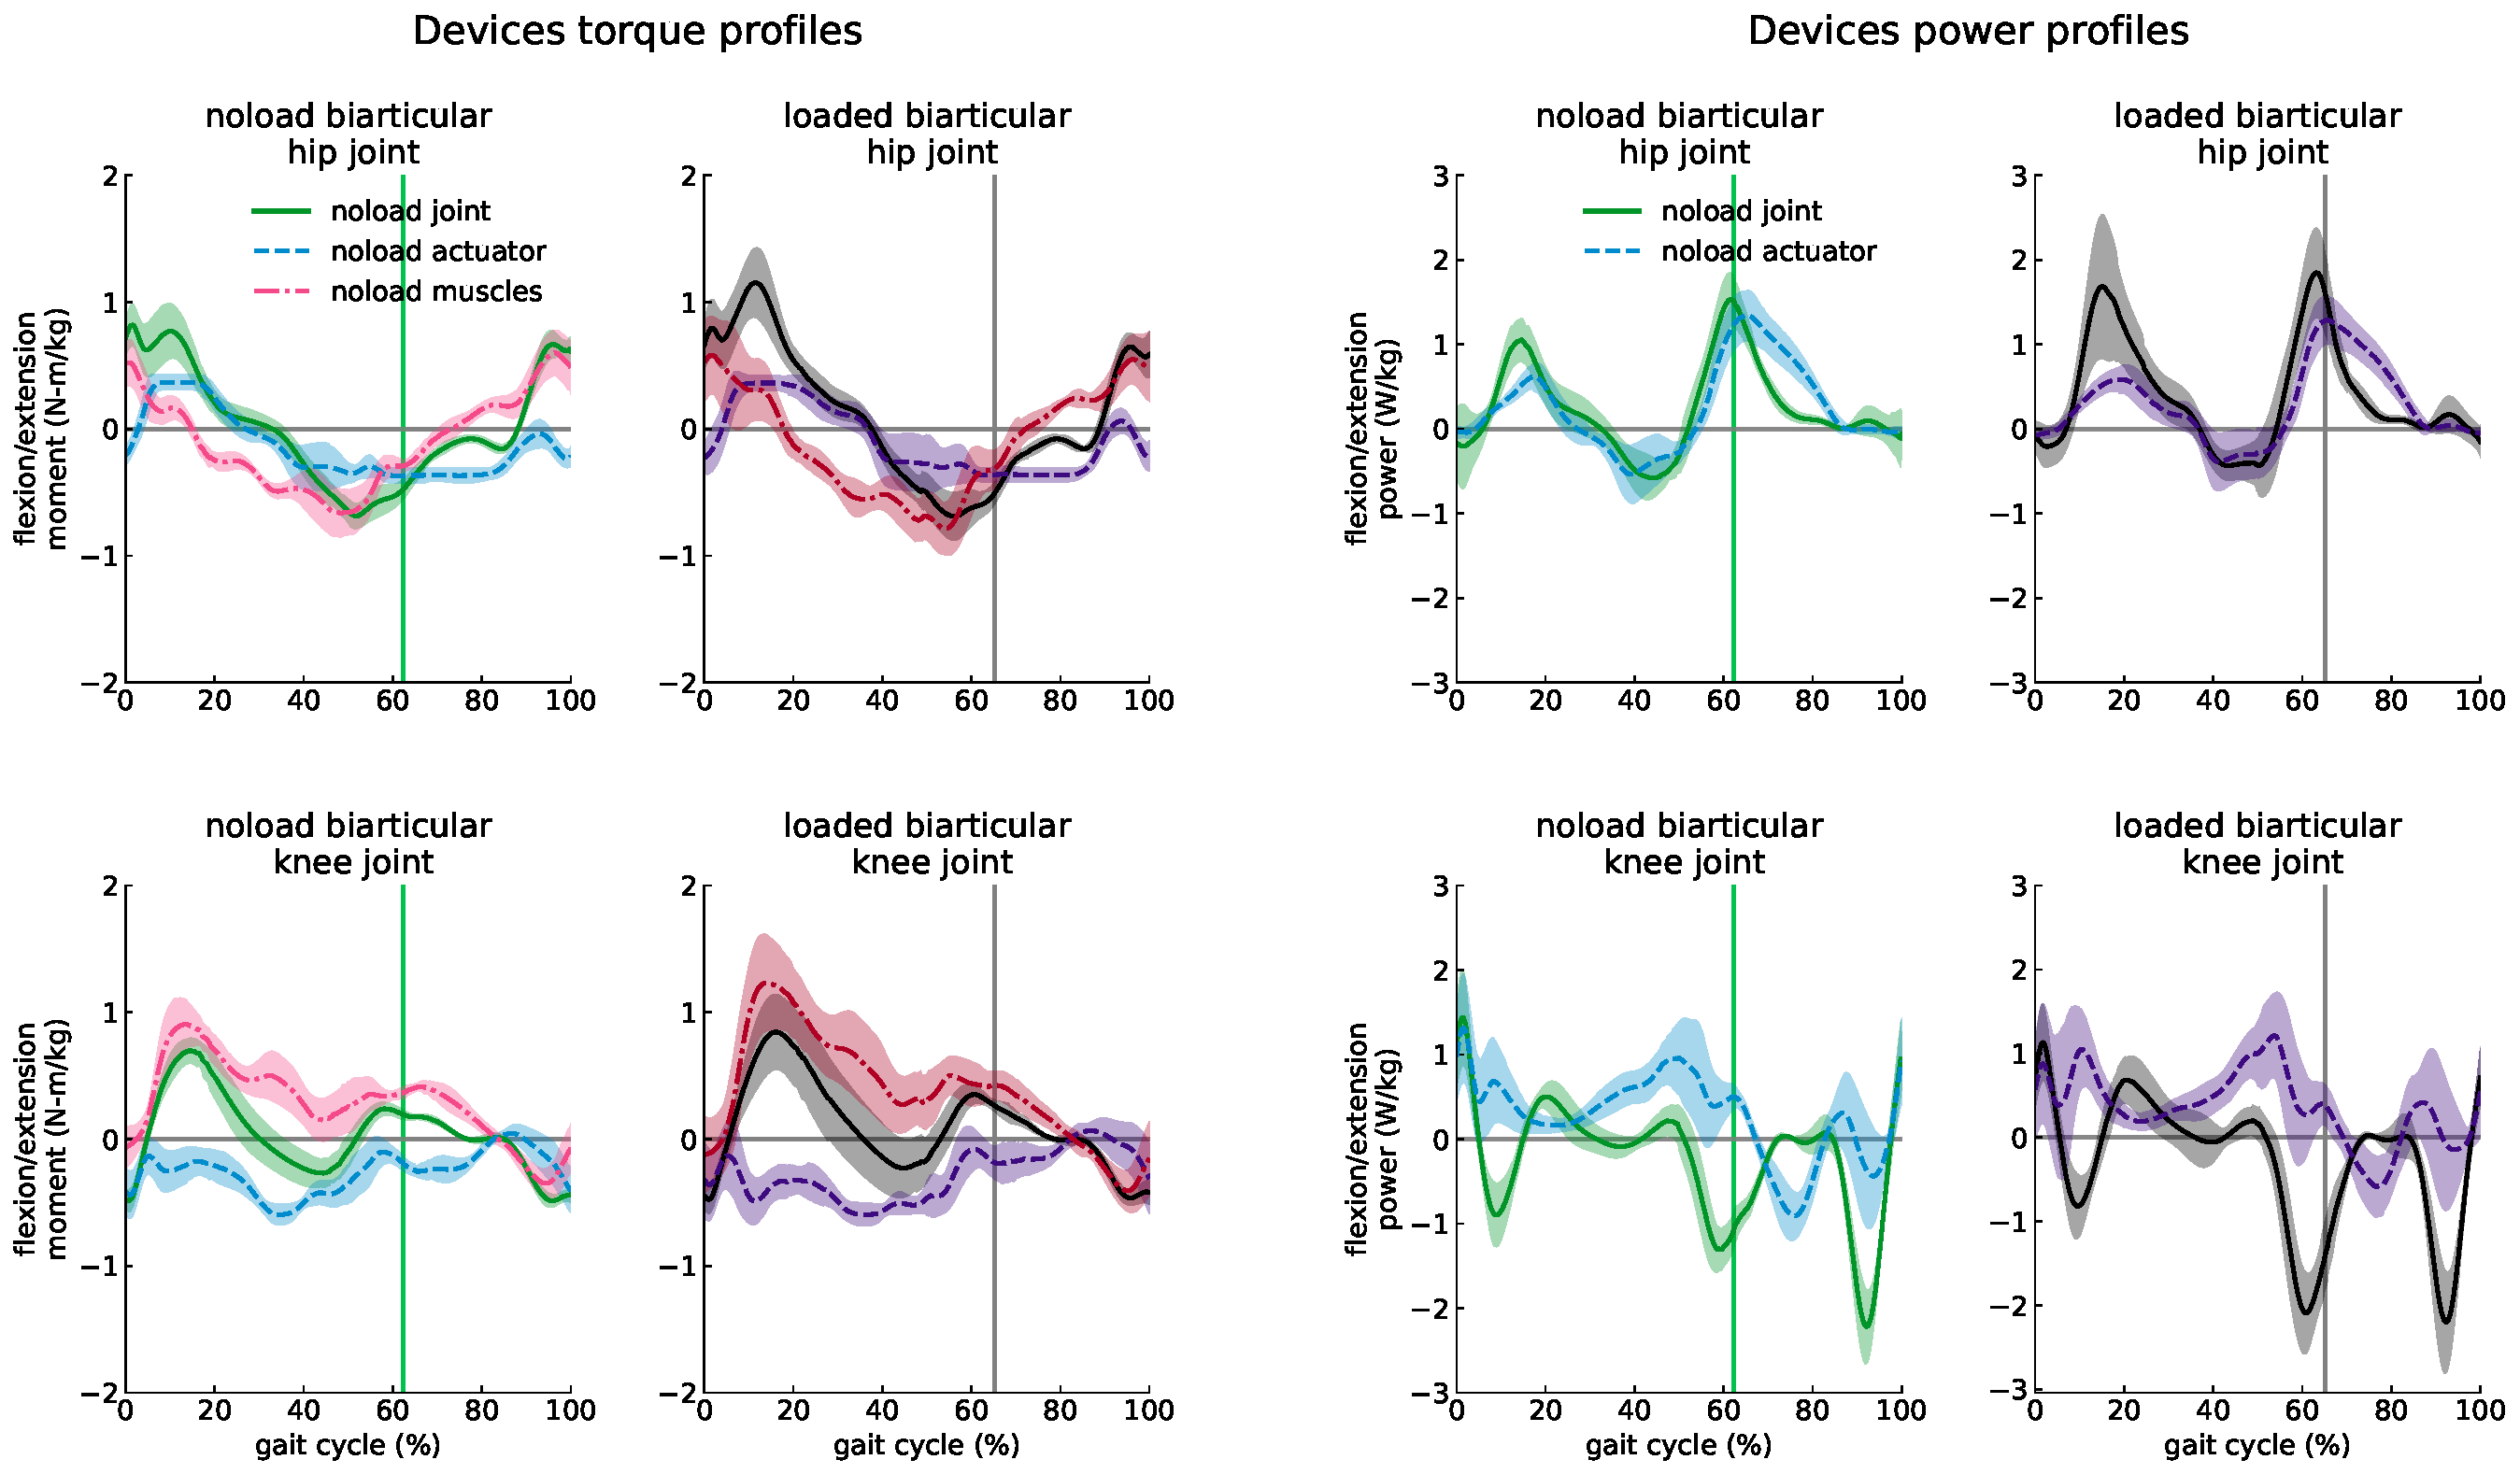
\includegraphics[width=\linewidth]{Case_Studies/NoloadBi23_LoadedBi23/PaperFigure_Profiles.pdf}
		\label{Fig_Case03_SamePowerConsumption}}
	\vspace{1mm}
	\caption{\small{\textbf{Biarticular exoskeleton actuators torque and power profiles and muscles generated moment of assisted subjects.} }}
	\label{Fig_Case03_Profiles}
\end{figure*}
The quantitative along with the qualitative analyses of power and moment profiles between pair of selected devices shows not only a moderate variation between the torque profiles of the compared biarticular devices but also the power profiles demonstrated considerably low diversity in different load conditions, as shown in Figure \ref{Fig_Case03_RMSE}\subref{Fig_Case03_RMSE_SameMetabolicConsumption}, \ref{Fig_Case03_RMSE}\subref{Fig_Case03_RMSE_SamePowerConsumption}. Additionally, Figure in \ref{Fig_Case03_Profiles} supports our claims on the high resemblance between profiles of the biarticular exoskeletons in the {\it loaded} and {\it noload} conditions. As shown in Figure \ref{Fig_Case03_Profiles}, the difference between the power and moment profiles of pair of devices in {\it load} and {\it noload} conditions were practically limited to the magnitude and timing based on the toe-off difference except on the pre-swing and initial-swing phases of knee profiles in where the trajectories had differences between biarticular devices with the same effect on the metabolic power consumption of assisted subjects.\\
%%%%%%%%%%%%%%%%%%%%%%%%%%%%%%%%%%%%%%%%%%%%%%%%%%%%%%%%%%%%%%%%%%%%%%%%%%%%%%%%%%%%%%%%%%%%%%%%%%%%%%%%%%%%%%%%%%%%
\section*{Case 4: Monoarticular Exoskeleton Performance} 
\begin{figure*}[ht!]
	\centering
	\subfloat[\small{Monoarticular exoskeleton with the same effect on the metabolic consumption of subjects}]{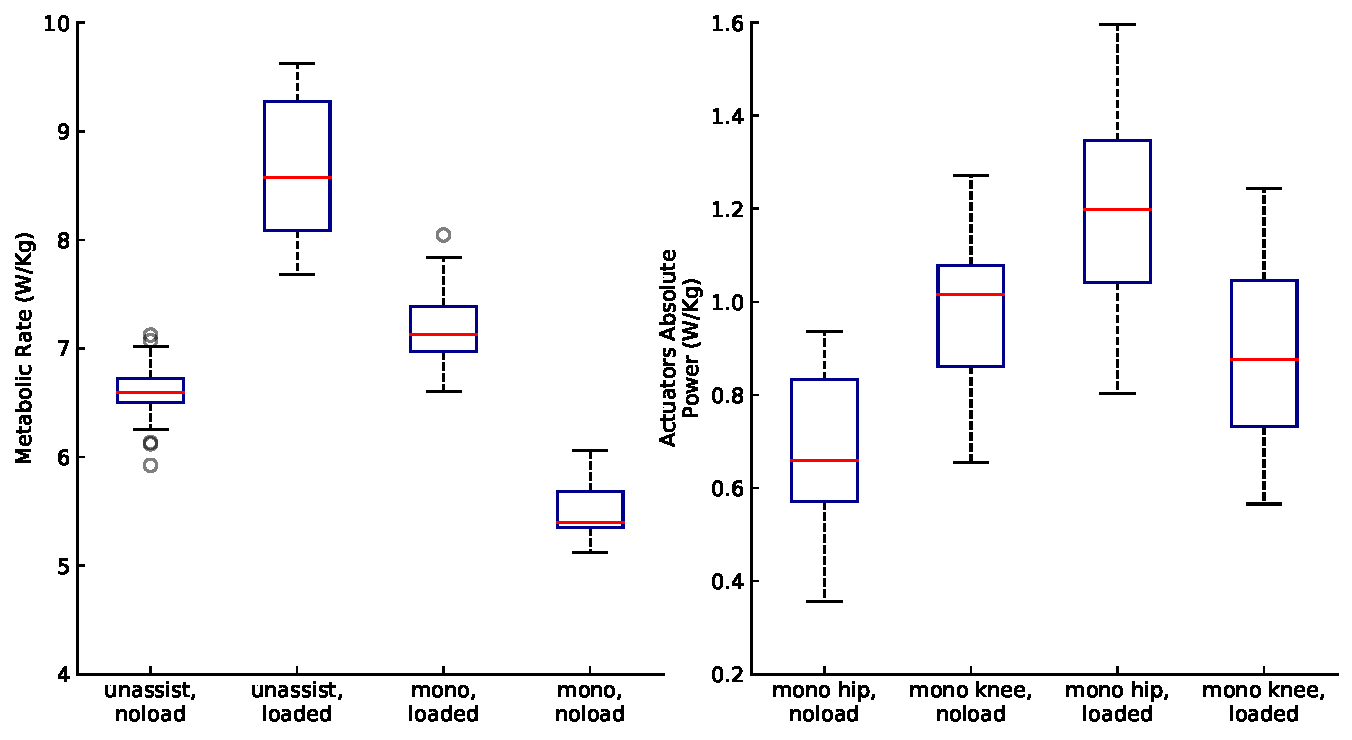
\includegraphics[width=\linewidth]{Case_Studies/NoloadMono25_LoadedMono05/PaperFigure_BoxPlot.pdf}
		\label{Fig_Case04_Energy_Plot_SameMetabolicConsumption}}
	\hfil
	\subfloat[\small{Monoarticular exoskeleton with the same total power consumptions }]{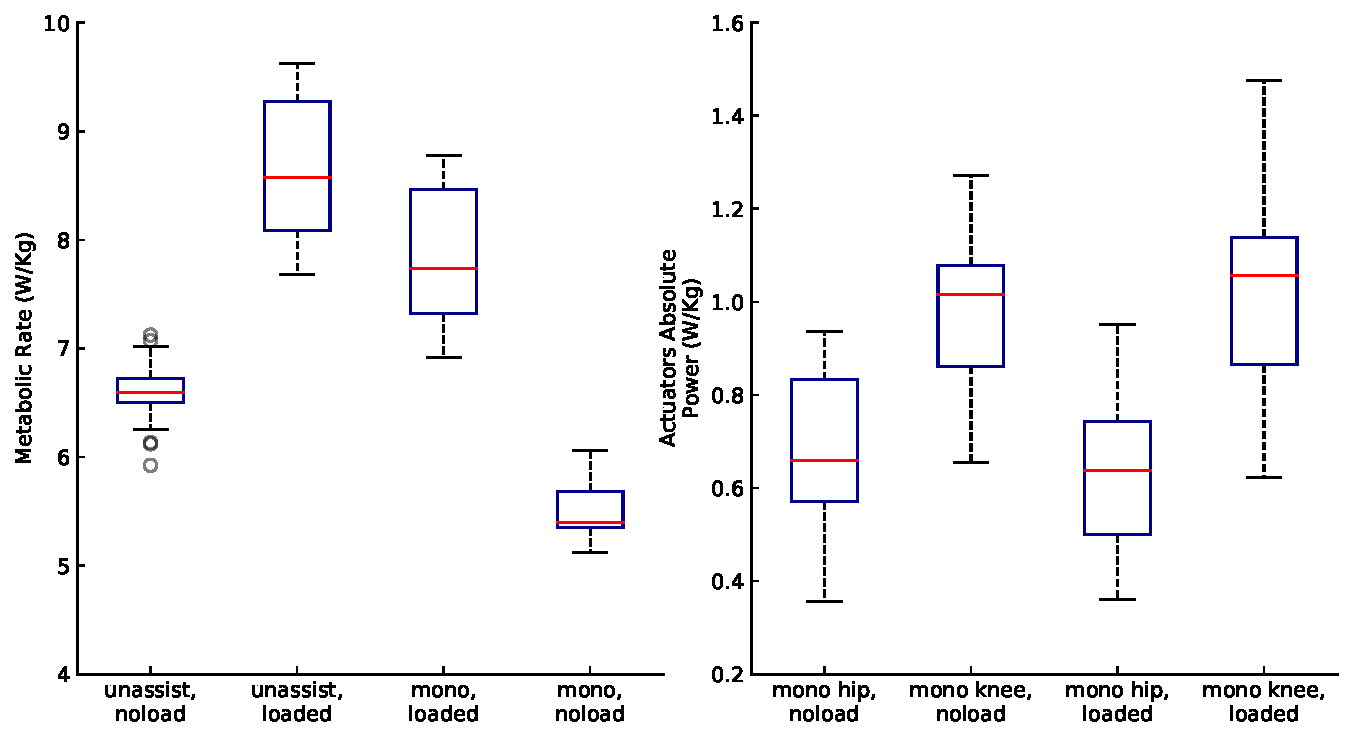
\includegraphics[width=\linewidth]{Case_Studies/NoloadMono25_LoadedMono25/PaperFigure_BoxPlot.pdf}
		\label{Fig_Case04_Energy_Plot_SamePowerConsumption}}
	\vspace{1mm}
	\caption{\small{\textbf{Monoarticular exoskeleton power consumption and its effect on the metabolic rate in different load conditions.} The power consumptions of biarticular exoskeleton and their effect on whole-body metabolic rate of the subjects walking at self-selected speed in both {\it loaded} and {\it noload} condition. Asterisks indicate statistically significant differences ( 7 subjects, 3 trails, Tukey Post-hoc, $P < 0.05$).}}
	\label{Fig_Case04_Energy_Plot}
\end{figure*}
\begin{figure*}[ht!]
	\centering
	\subfloat[\small{Monoarticular exoskeleton with the same effect on the metabolic consumption of subjects}]{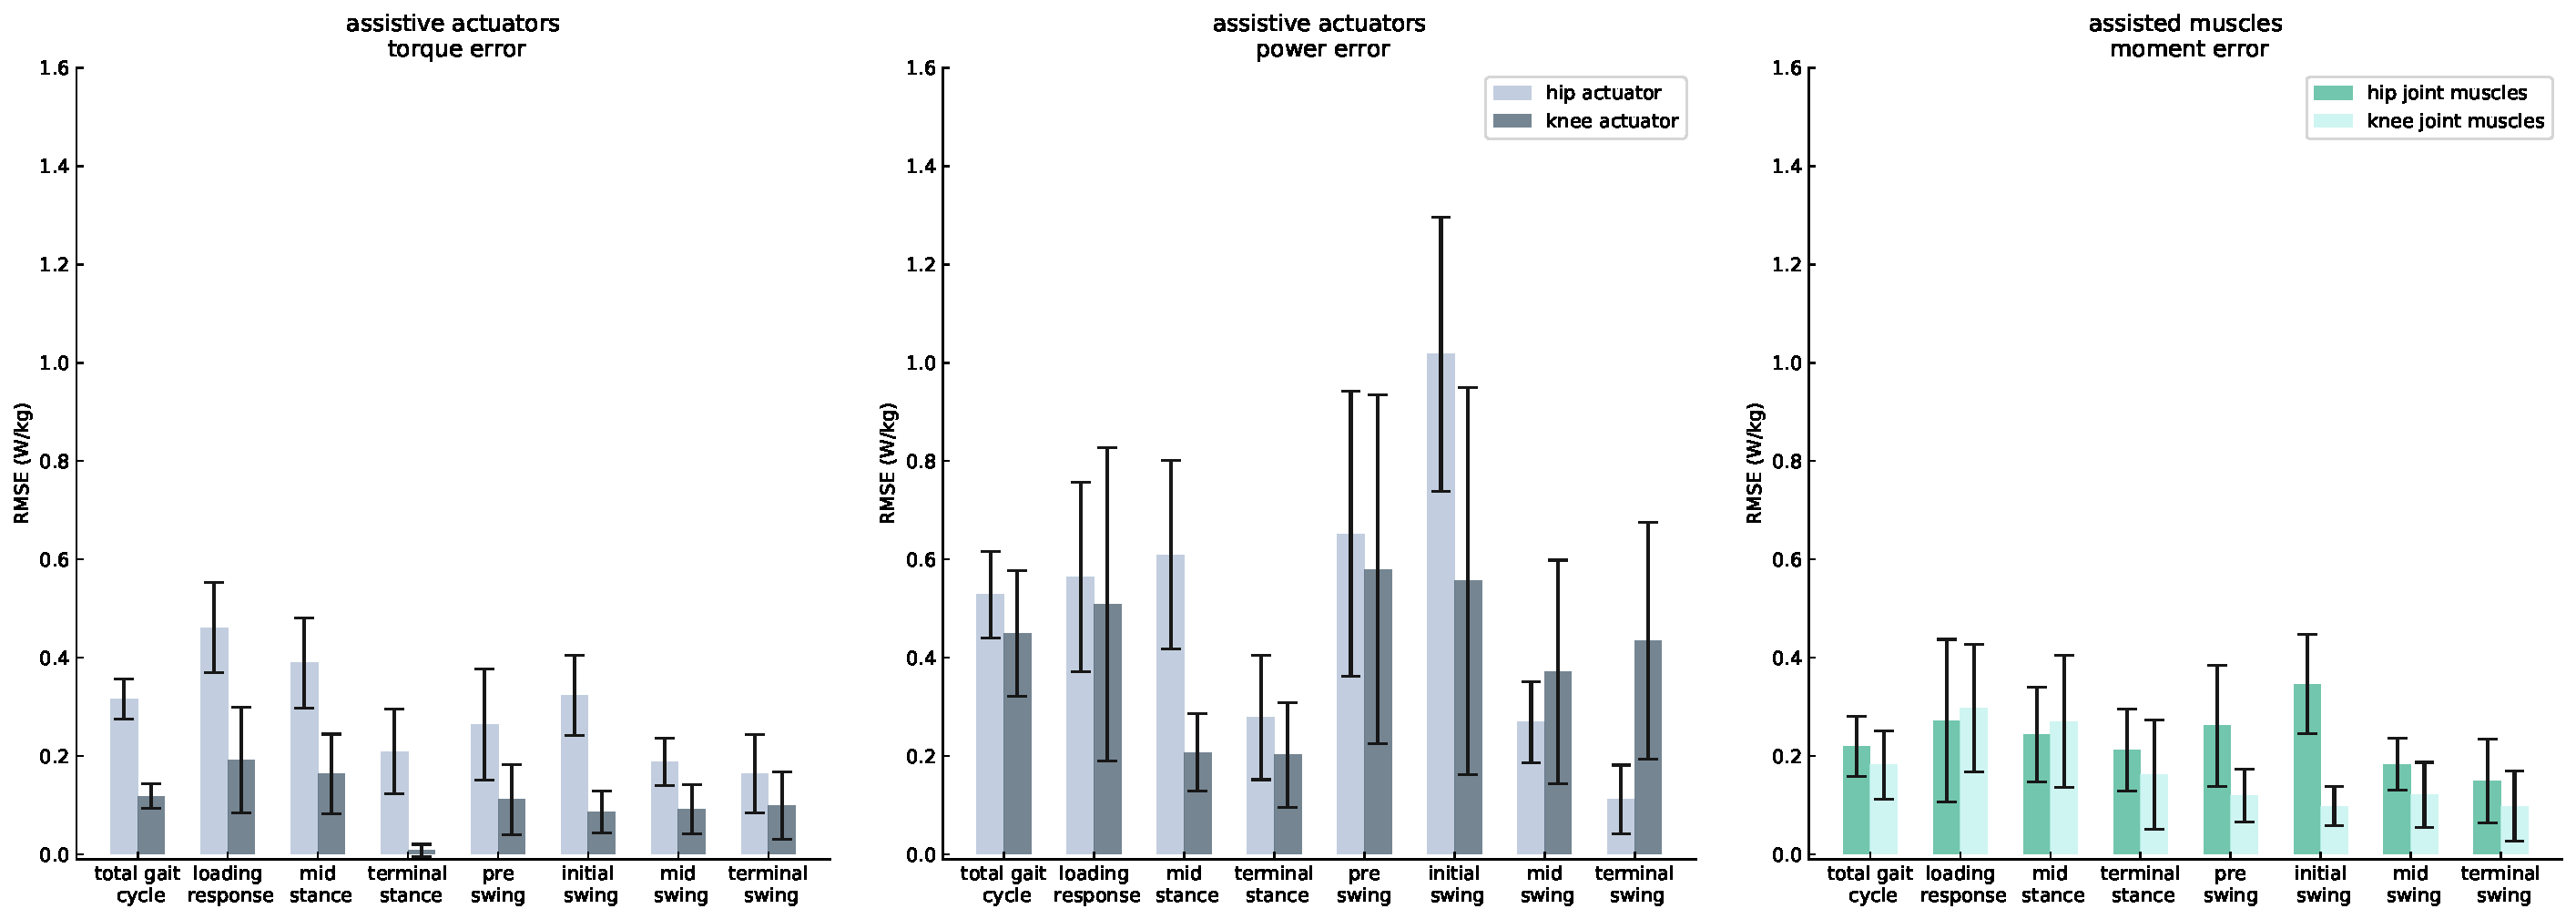
\includegraphics[width=\linewidth]{Case_Studies/NoloadMono25_LoadedMono05/RMSE.pdf}
		\label{Fig_Case04_RMSE_SameMetabolicConsumption}}
	\hfil
	\subfloat[\small{Monoarticular exoskeleton with the same total power consumptions }]{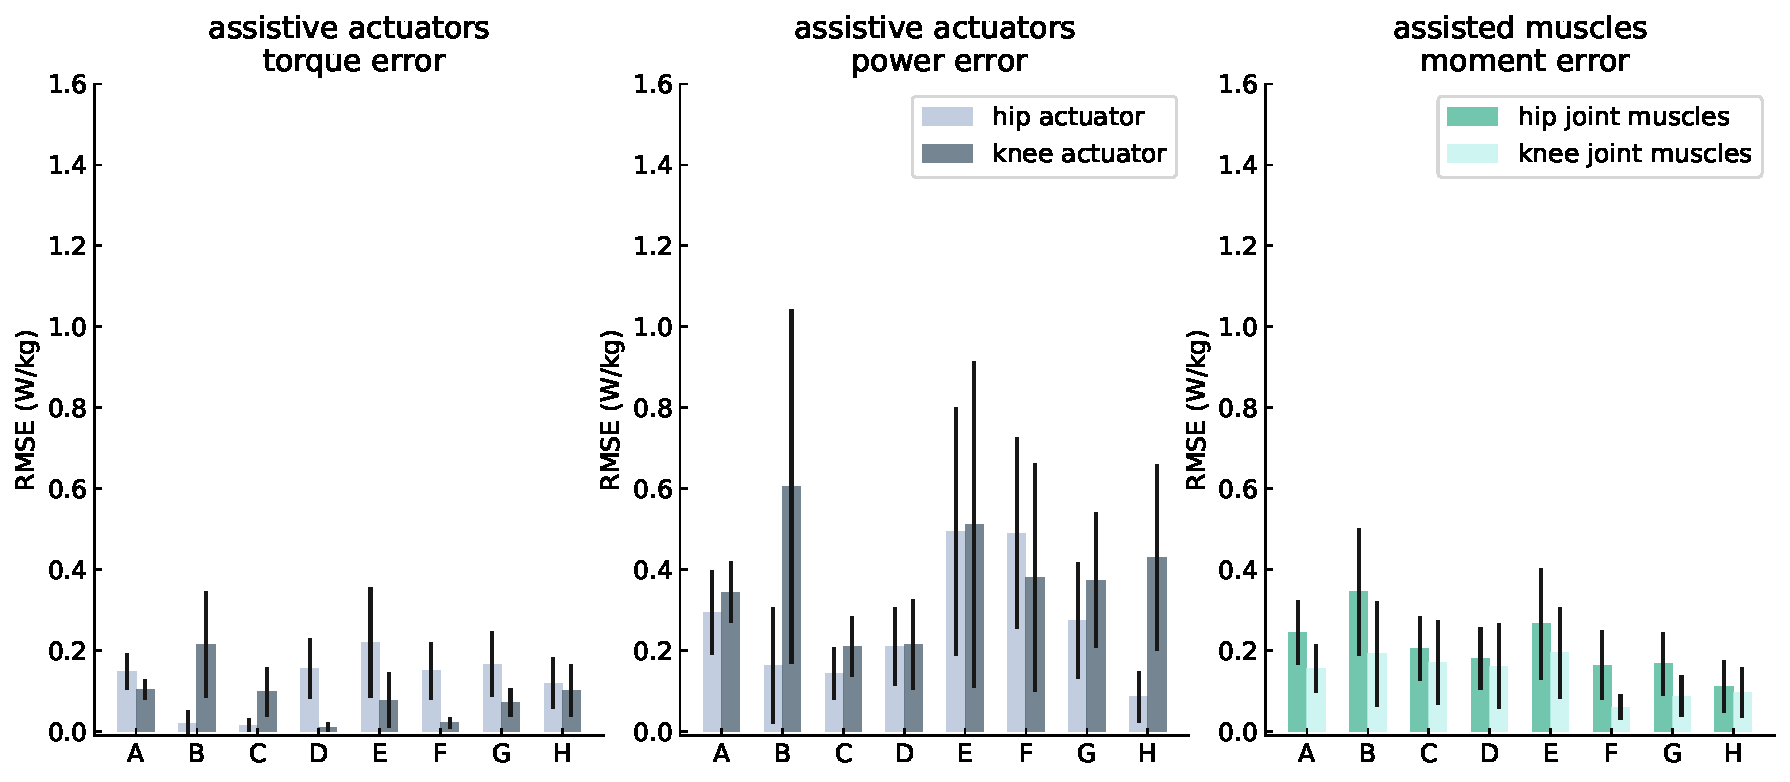
\includegraphics[width=\linewidth]{Case_Studies/NoloadMono25_LoadedMono25/RMSE.pdf}
		\label{Fig_Case04_RMSE_SamePowerConsumption}}
	\vspace{1mm}
	\caption{\small{\textbf{Monoarticular exoskeleton torque and power and muscles generated moment profiles root mean square error in different load conditions.} The root mean square error between actuators of the biarticular exoskeleton and the muscles generated moment of subjects assisted by this device {\it loaded} and {\it noload} conditions.}}
	\label{Fig_Case04_RMSE}
\end{figure*}
The same analyses on the biarticular exoskeleton in different load conditions, which was discussed in the previous case study,  were performed on the monoarticular exoskeleton to gain an in-depth insight into this device. To conduct the comparisons between a pair of monoarticular devices with a similar effect on the metabolic cost or with similar power consumption, we chose the "Ee" configuration of monoarticular in loaded and noload conditions and "Ae" monoarticular exoskeleton from the Pareto front of the monoarticular in the loaded condition. The selected "Ee" and "Ae" configurations have 30 and 30 N-m, and 70 and 30 N-m peak torque constraints on the pair of hip and knee actuators.\\
The comparison of actuators power consumption between the "Ae" {\it loaded} and "Ee" {\it noload}, which have a similar metabolic cost reduction, showed a notable increase in power consumption of the {\it loaded} hip actuator. Despite the reduction in the knee power consumption of {\it loaded} knee actuator, the difference between the pair knee actuators was not significant. One of the observed critical issues was that even though the within-subject variation of monoarticular devices was generally low, the deviation of actuators power consumption between the load condition and between the configurations was considerably high. As shown in Figure \ref{Fig_Case04_Energy_Plot}\subref{Fig_Case04_Energy_Plot_SameMetabolicConsumption} along with Figure \ref{Fig_Case04_Energy_Plot}\subref{Fig_Case04_Energy_Plot_SamePowerConsumption}, while the power consumption of knee actuator in the low torque availability (i.e., "Ee") was higher than the hip actuator, this was changed in higher torque constraints, and the hip actuator became dominant power consumer indicating considerable changes in the power profile of monoarticular device in different arrangements of its actuators.\\
\begin{figure*}[ht!]
	\centering
	\subfloat[\small{Monoarticular exoskeleton with the same effect on the metabolic consumption of subjects}]{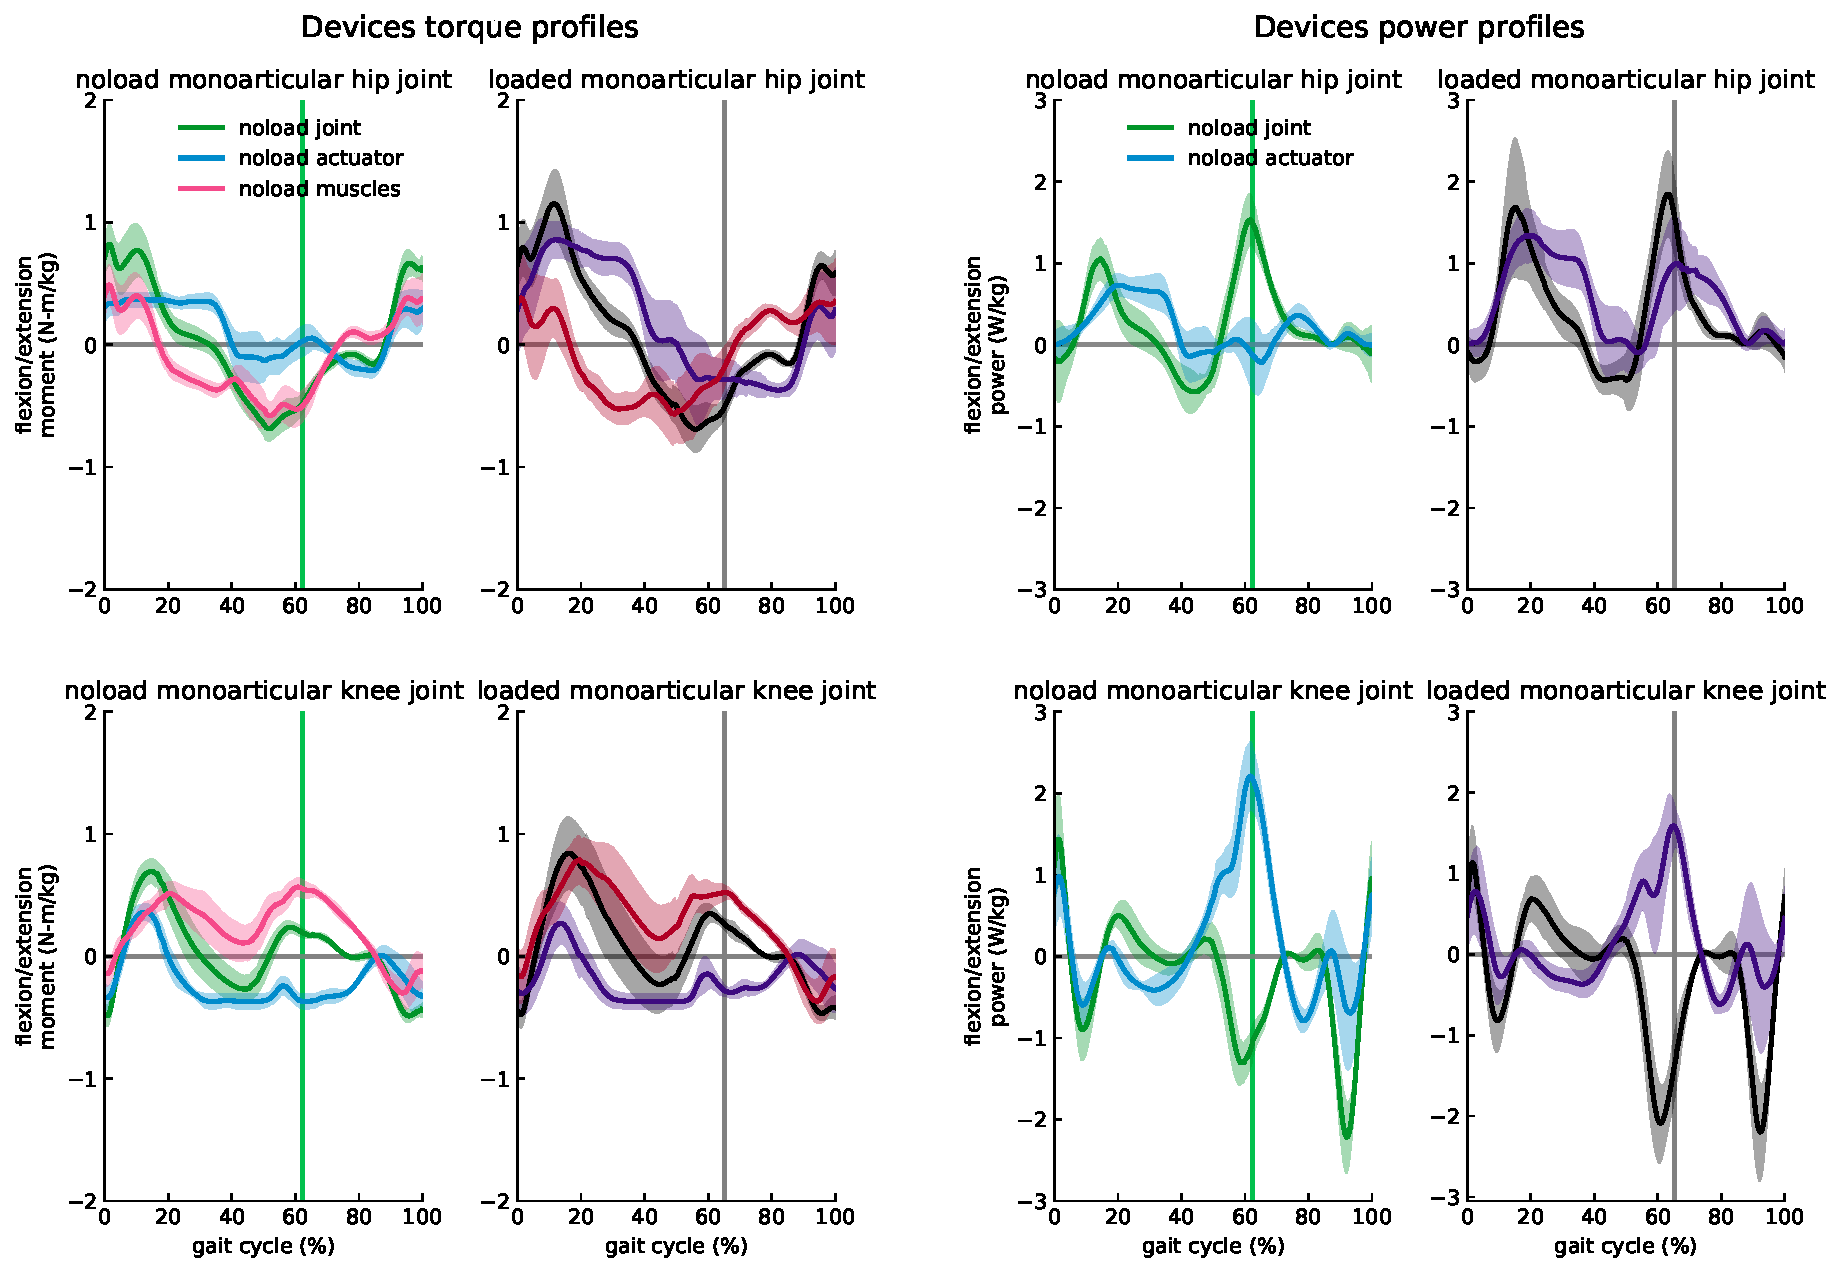
\includegraphics[width=\linewidth]{Case_Studies/NoloadMono25_LoadedMono05/PaperFigure_Profiles.pdf}
		\label{Fig_Case04_SameMetabolicConsumption}}
	\hfil
	\subfloat[\small{Monoarticular exoskeleton with the same total power consumptions }]{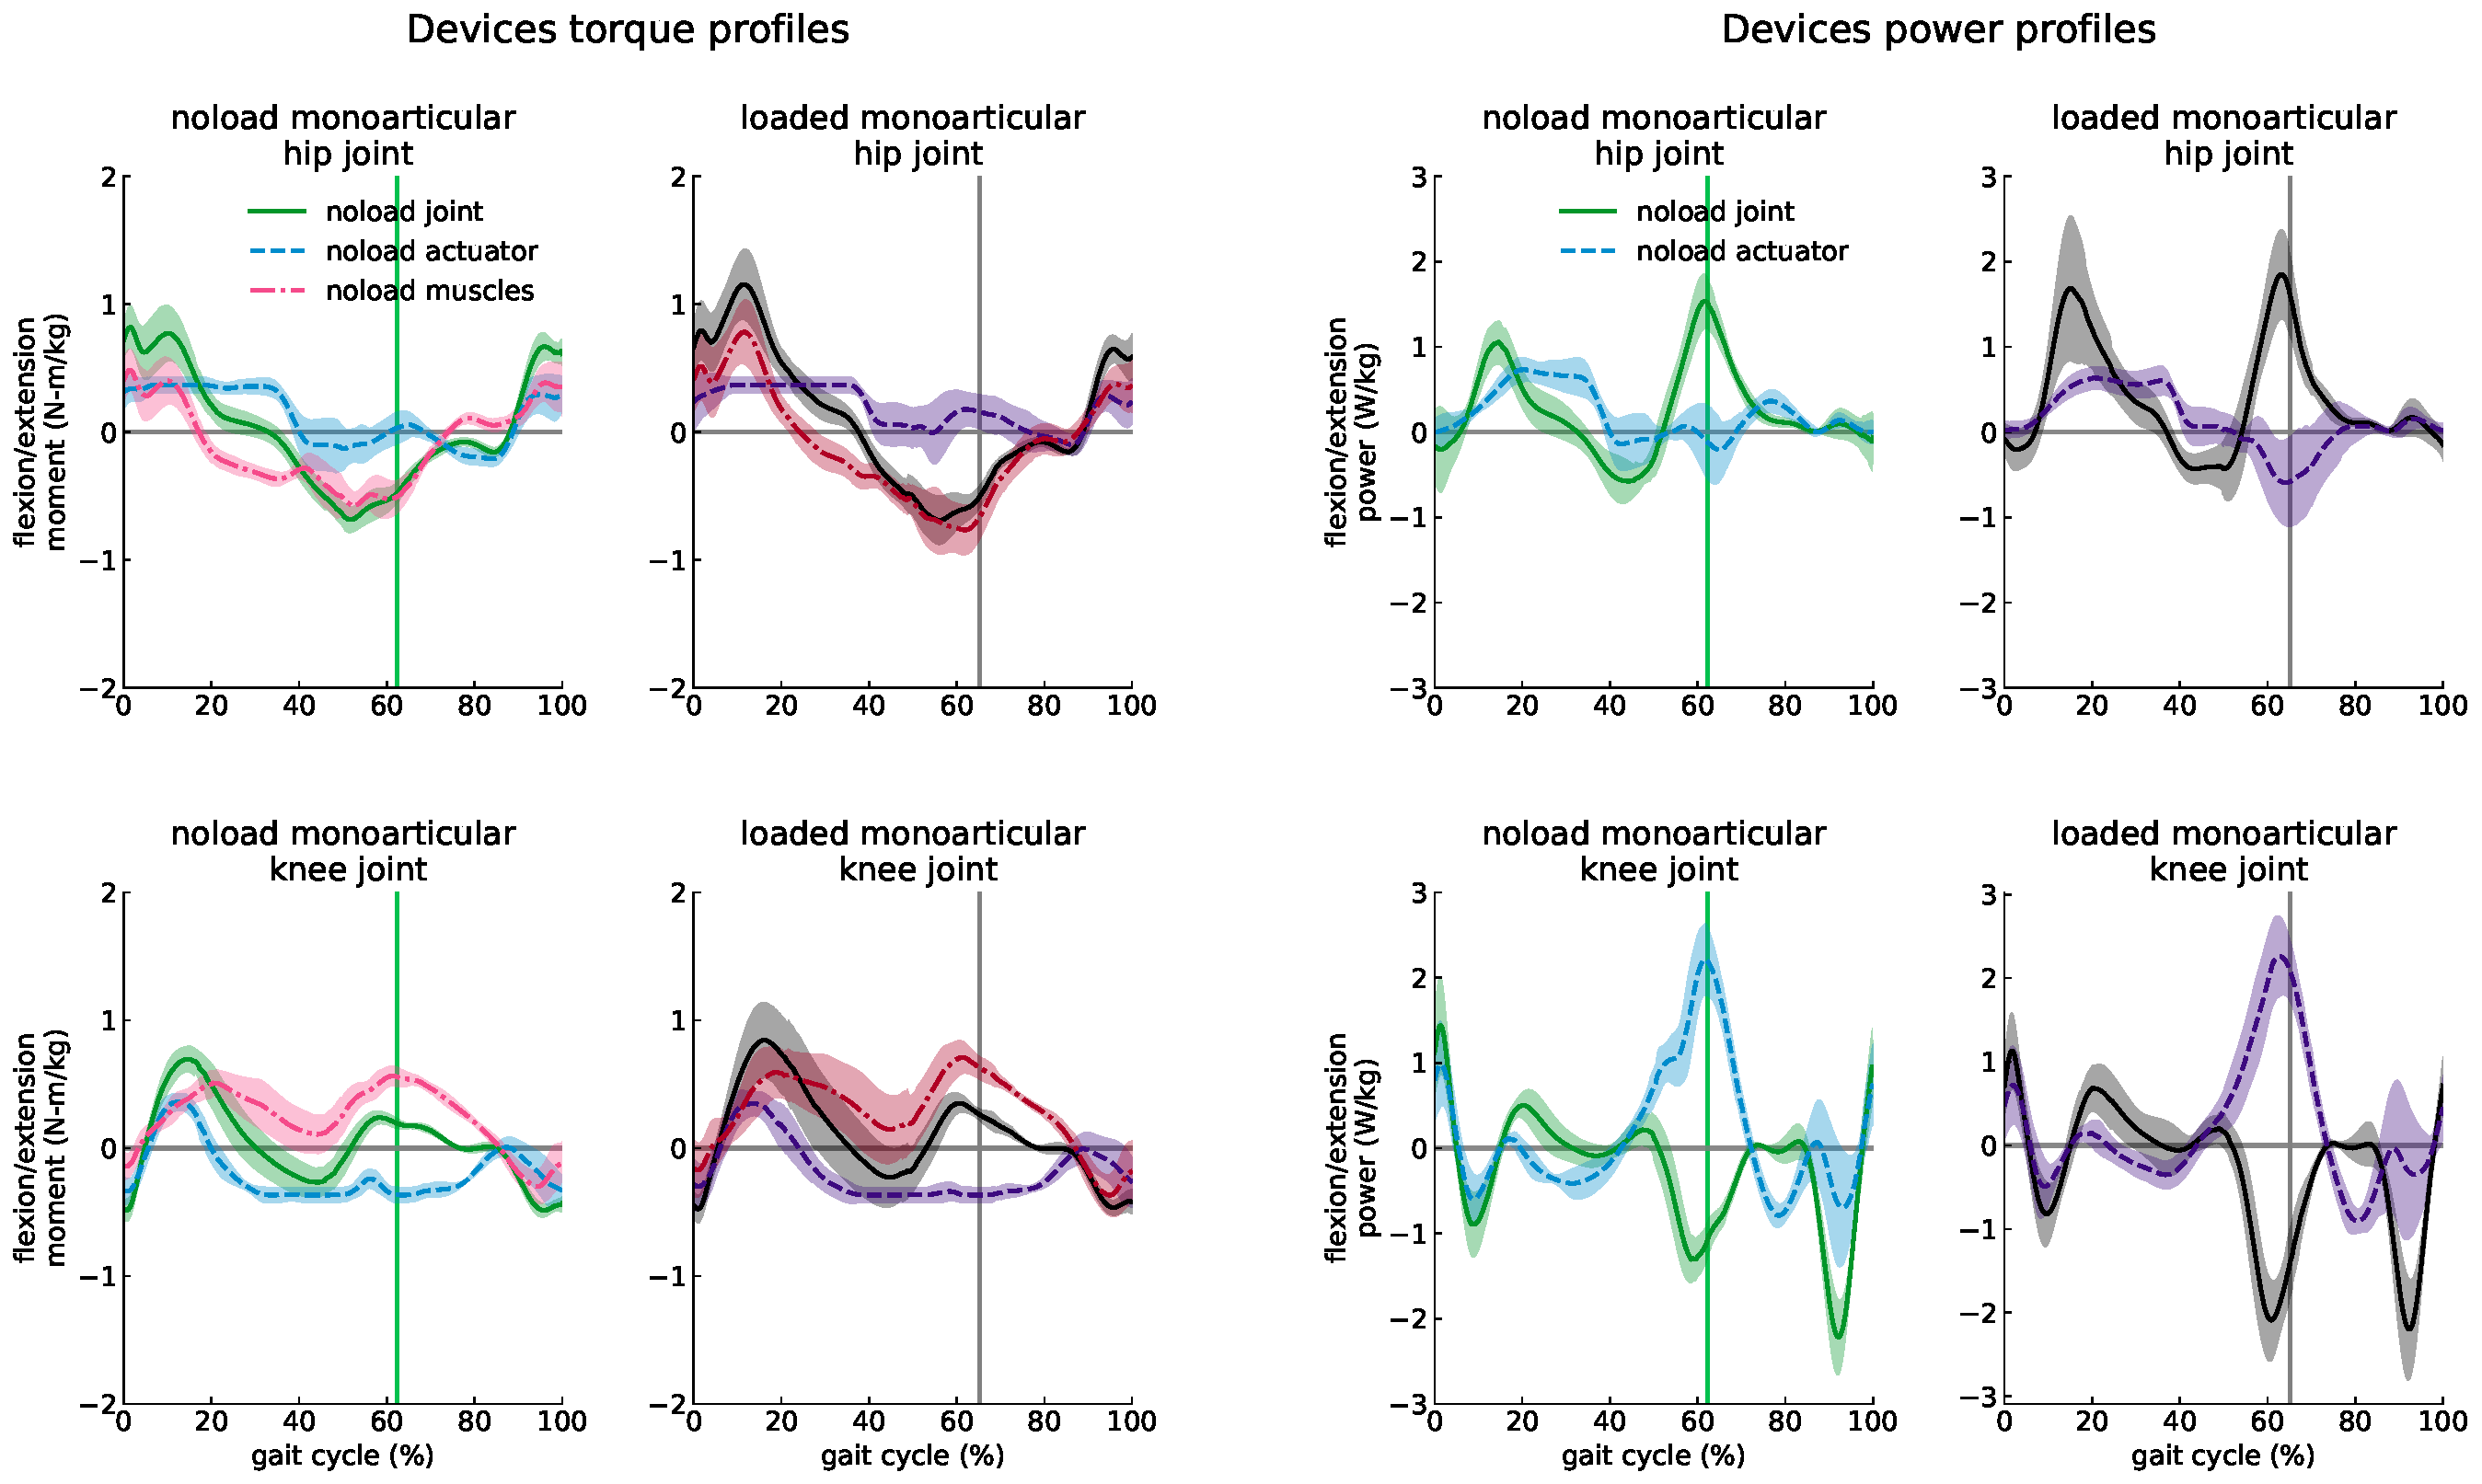
\includegraphics[width=\linewidth]{Case_Studies/NoloadMono25_LoadedMono25/PaperFigure_Profiles.pdf}
		\label{Fig_Case04_SamePowerConsumption}}
	\vspace{1mm}
	\caption{\small{\textbf{Monoarticular exoskeleton actuators torque and power profiles and muscles generated moment of assisted subjects.} }}
	\label{Fig_Case04_Profiles}
\end{figure*}
The metabolic rate of the compared pairs of monoarticular devices was shown in Figures \ref{Fig_Case04_Energy_Plot}\subref{Fig_Case04_Energy_Plot_SameMetabolicConsumption} and \ref{Fig_Case04_Energy_Plot}\subref{Fig_Case04_Energy_Plot_SamePowerConsumption}. These figures showed similar behavior observed in the previous case study. However, it is noteworthy to mention the significant difference between the impact of the "Ee" device on the metabolic burden reduction of subjects in different loading conditions, which we did not observe in the biarticular case. These high deviations in both defined performance criteria can complicate obtaining a general exoskeleton that can deliver different levels of assistance with efficient power consumption.\\
The pair of devices selected for conducting the comparisons were evaluated by the modified augmentation factor to assess their performance under their mass and inertia effect. Unlike the other case studies in which all evaluated biarticular and monoarticular devices were delivering a positive power to the human musculoskeletal system, the monoarticular exoskeletons evaluated in this case study both were causing an increase in the metabolic expenditure of subjects according to MAF performance factor. The modified augmentation factor of the monoarticular device with 30 N-m peak torque constraints in both hip and knee actuators showed -0.20 $\pm$ 0.43 W/kg in the {\it noload} condition while it was increased to -0.15 $\pm$ 0.56 W/kg when subjects were loaded. These MAF values of the "Ee" monoarticular device represent a high variation of device effect on the subjects and improvement of the device performance by loading subjects, which was also observed in the biarticular exoskeleton. Even with the improvement of device performance in the loaded condition, the device in both loading conditions would cause subjects to consume more power due to wearing these devices. The same analysis on the monoarticular device "Ae" configuration (70 N-m hip 30 N-m knee) in {\it loaded} condition showed relative improvement compared to the "Ee" device.\\
According to the MAF value, the monoarticular exoskeleton requires a large torque capacity at the hip actuator to deliver assistance to the subjects. According to the slope of Pareto front of monoarticular device under the devices inertial properties effect, we claimed that it might be beneficial to keep the torque capacity of the monoarticular exoskeleton more moderate, yet, we observe in this case study that the monoarticular device cannot inject positive power to the human musculoskeletal system in low torque capacity. According to the MAF value and our previous observations, it might be reasonable to conclude that designing an optimal monoarticular exoskeleton that can be used for different assistance levels and load conditions is complicated.\\
The moment and power profiles of the selected monoarticular exoskeleton did not show a similar resemblance that we observed in the biarticular device between the pair of actuators. The hip actuators of devices with the same metabolic reduction effect followed completely different trajectories, and it was not surprising that their power profiles had significant differences. Although the moment profiles of the knee actuators had a higher resemblance than the hip actuators, their power profiles showed relatively different paths during pre-swing and initial swing phases. The comparison of the same device ( i.e., "Ee") profiles in different load conditions showed a considerable divergence between the profiles of the hip actuator after the mid-stance phase of the gait cycle and their maximum difference occurred during the pre-swing and initial swing phases. Although the knee actuators showed similar torque profiles in different load conditions, their power profiles demonstrated remarkable differences during pre-swing and initial swing phases. These described moment and power profiles and their quantitative differences, using the RMSE, in both comparison cases are represented in Figures \ref{Fig_Case04_Profiles} and \ref{Fig_Case04_RMSE}.\\
This case study confirms our discussion about monoarticular exoskeleton in which we claimed that obtaining a generic control policy for this device would be challenging. Also, designing an optimal battery under its life and weight considerations highly depends on the selected configuration, and a generic battery would not perform optimally for the monoarticular device in different assistance levels and load conditions.
\end{document}
